\documentclass[12pt,twoside,a4paper]{report}
\usepackage{etex}
% Select encoding of your inputs.
\usepackage[utf8]{inputenc}

% Make latex understand and use the typographic
% rules of the language used in the document.
\usepackage[english, danish]{babel}

% Use the vector font Latin Modern which is going
% to be the default font in latex in the future.
\usepackage{lmodern}

% Choose the font encoding
\usepackage[T1]{fontenc}

% Use colour in tables
\usepackage[table]{xcolor}

\usepackage{array}

\usepackage{multirow}

% load a colour package
\usepackage{xcolor}
\definecolor{aaublue}{RGB}{33,26,82}% dark blue

% The standard graphics inclusion package
\definecolor{white}{RGB}{255,255,255} % define color white
\usepackage{graphicx}
\usepackage{adjustbox}

% Set up how figure and table captions are displayed
\usepackage{caption}
\captionsetup{%
  font=footnotesize,% set font size to footnotesize
  labelfont=bf % bold label (e.g., Figure 3.2) font
}

% Enable row combination in tables
\usepackage{multirow}

% Make space between table lines and text
\renewcommand{\arraystretch}{1.5}

% Make the standard latex tables look so much better
\usepackage{array,booktabs}

% Enable the use of frames around, e.g., theorems
% The framed package is used in the example environment
\usepackage{framed}
\usepackage{colortbl}
\usepackage{longtable}
\usepackage{xcolor}

\usepackage{textcomp}

%%%%%%%%%%%%%%%%%%%%%%%%%%%%%%%%%%%%%%%%%%%%%%%%
% Mathematics
%%%%%%%%%%%%%%%%%%%%%%%%%%%%%%%%%%%%%%%%%%%%%%%%
% Defines new environments such as equation,
% align and split 
\usepackage{amsmath}
\usepackage{relsize}
% Adds new math symbols
\usepackage{amssymb}
% Use theorems in your document
% The ntheorem package is also used for the example environment
% When using thmmarks, amsmath must be an option as well. Otherwise \eqref doesn't work anymore.
\usepackage[framed,amsmath,thmmarks]{ntheorem}

%%%%%%%%%%%%%%%%%%%%%%%%%%%%%%%%%%%%%%%%%%%%%%%%
% Page Layout
%%%%%%%%%%%%%%%%%%%%%%%%%%%%%%%%%%%%%%%%%%%%%%%%
% Change margins, papersize, etc of the document
\usepackage[
  left=25mm,% left margin on an odd page %tidligere 25mm for baade right og left
  right=25mm,% right margin on an odd page
  top=35mm,
  ]{geometry}
  
% Modify how \chapter, \section, etc. look
% The titlesec package is very configureable
\usepackage{titlesec}
\makeatletter
\def\ttl@mkchap@i#1#2#3#4#5#6#7{%
    \ttl@assign\@tempskipa#3\relax\beforetitleunit
    \vspace{\@tempskipa}%<<<<<< REMOVE THE * AFTER \vspace
    \global\@afterindenttrue
    \ifcase#5 \global\@afterindentfalse\fi
    \ttl@assign\@tempskipb#4\relax\aftertitleunit
    \ttl@topmode{\@tempskipb}{%
        \ttl@select{#6}{#1}{#2}{#7}}%
    \ttl@finmarks  % Outside the box!
    \@ifundefined{ttlp@#6}{}{\ttlp@write{#6}}}
\makeatother

\titlespacing{\chapter}{0pt}{0pt}{10pt}
\titlespacing{\section}{0pt}{0pt}{-5pt}
\titlespacing{\subsection}{0pt}{8pt}{-5pt}
\titlespacing{\subsubsection}{0pt}{6pt}{-10pt}

\titleformat*{\section}{\normalfont\Large\bfseries\color{aaublue}}
\titleformat*{\subsection}{\normalfont\large\bfseries\color{aaublue}}
\titleformat*{\subsubsection}{\normalfont\normalsize\bfseries\color{aaublue}}
%\titleformat*{\paragraph}{\normalfont\normalsize\bfseries\color{aaublue}}
%\titleformat*{\subparagraph}{\normalfont\normalsize\bfseries\color{aaublue}}

%Formatting chapter headers. Predefined styles that can be used as option to the package: Sonny, Lenny, Glenn, Conny, Rejne, Bjarne, PetersLenny and Bjornstrup

%\usepackage[Sonny]{fncychap}

\usepackage{titlesec, blindtext, color}
%\color{gray75}{gray}{0.75}
\newcommand{\hsp}{\hspace{20pt}}
\titleformat{\chapter}[hang]{\Huge\bfseries}{\thechapter\hsp\textcolor{aaublue}{|}\hsp}{0pt}{\Huge\bfseries}


% Change the headers and footers
\usepackage{fancyhdr}
\setlength{\headheight}{15pt}
\pagestyle{fancy}
\fancyhf{} %delete everything
\renewcommand{\headrulewidth}{0pt} %remove the horizontal line in the header
\fancyhead[RO,LE]{\color{aaublue}\small\nouppercase\leftmark} %even page - chapter title

\fancyhead[LO]{}
\fancyhead[RE]{} 
\fancyhead[CE]{}
\fancyhead[CO]{}

\fancyfoot[RE,LO]{\thepage}
\fancyfoot[LE,RO]{B205} %page number on all pages
\fancyfoot[CE,CO]{}



% change first page of all chapters header and footer to fancy style
\makeatletter
\let\ps@plain\ps@fancy
\makeatother

% Do not stretch the content of a page. Instead,
% insert white space at the bottom of the page
\raggedbottom

% Enable arithmetics with length. Useful when typesetting the layout.
\usepackage{calc}

%%%%%%%%%%%%%%%%%%%%%%%%%%%%%%%%%%%%%%%%%%%%%%%%
% Bibliography
%%%%%%%%%%%%%%%%%%%%%%%%%%%%%%%%%%%%%%%%%%%%%%%%
%setting references (using numbers) and supporting i.a. Chicargo-style:
\usepackage{etex}
\usepackage{etoolbox}
\usepackage{keyval}
\usepackage{ifthen}
\usepackage{url}
\usepackage{csquotes}
\usepackage[backend=biber, url=true, doi=true, style=numeric, sorting=none]{biblatex}
\addbibresource{setup/bibliography.bib}




%% Add the \citep{key} command which display a
%% reference as [author, year]
%\usepackage[square]{natbib}
%\usepackage{natbib}
%% Appearance of the bibliography
%\bibliographystyle{setup/apalike}
%%\bibliographystyle{IEEEtran}

%%%%%%%%%%%%%%%%%%%%%%%%%%%%%%%%%%%%%%%%%%%%%%%%
% Misc
%%%%%%%%%%%%%%%%%%%%%%%%%%%%%%%%%%%%%%%%%%%%%%%%

% Add bibliography and index to the table of
% contents
% %\usepackage[nottoc, notlof, notlot]{tocbibind}
\usepackage{tocloft}
% Add the command \pageref{LastPage} which refers to the
% page number of the last page
\setlength{\cftbeforetoctitleskip}{0 cm}

\usepackage[
  %disable, %turn off todonotes
  colorinlistoftodos, %enable a coloured square in the list of todos
  %inline,
  textwidth=\marginparwidth, %set the width of the todonotes
  textsize=scriptsize, %size of the text in the todonotes
  ]{todonotes}
    
\usepackage{wrapfig}
% Enables figures with text wrapped tightly around it 

%%% Section debth included in table of contents (1 = down to sections) %%%
\setcounter{tocdepth}{1}

%%% Section debth for numbers (1 = down to sections) %%%
\setcounter{secnumdepth}{1}

\renewcommand{\cftpartpresnum}{Part~}
\let\cftoldpartfont\cftpartfont
\renewcommand{\cftpartfont}{\cftoldpartfont\cftpartpresnum}

%%%%%%%%%%%%%%%%%%%%%%%%%%%%%%%%%%%%%%%%%%%%%%%%
% Hyperlinks
%%%%%%%%%%%%%%%%%%%%%%%%%%%%%%%%%%%%%%%%%%%%%%%%

% Enable hyperlinks and insert info into the pdf
% file. Hypperref should be loaded as one of the 
% last packages
\usepackage{nameref}
\usepackage{hyperref}
\hypersetup{%
	%pdfpagelabels=true,%
	plainpages=false,%
	pdfauthor={Author(s)},%
	pdftitle={Title},%
	pdfsubject={Subject},%
	bookmarksnumbered=true,%
	colorlinks,%
	citecolor=aaublue,%
	filecolor=aaublue,%
	linkcolor=aaublue,% you should probably change this to black before printing
	urlcolor=aaublue,%
	pdfstartview=FitH%
}

% remove all indentations
\setlength\parindent{0pt}
\parskip 5mm
\usepackage{verbatim}

\definecolor{Gra}{RGB}{230,230,230}

%creates a nice-looking C#-text
\newcommand{\CC}{C\nolinebreak\hspace{-.05em}\raisebox{.3ex}{\scriptsize\text \#} }

%enables multi column lists
\usepackage{multicol}

%enables code-examples
\usepackage{listings}

\definecolor{coolblue}{RGB}{32,95,128}
\definecolor{mygreen}{rgb}{0,0.6,0}
\definecolor{mygray}{rgb}{0.5,0.5,0.5}
\definecolor{mymauve}{rgb}{0.58,0,0.82}
\usepackage{textcomp}
\definecolor{listinggray}{gray}{0.9}
\definecolor{lbcolor}{rgb}{0.9,0.9,0.9}

\lstset{
%  backgroundcolor=\color{white},   % choose the background color; you must add \usepackage{color} or \usepackage{xcolor}
%  basicstyle=\footnotesize,        % the size of the fonts that are used for the code
%  breakatwhitespace=false,         % sets if automatic breaks should only happen at whitespace
%  breaklines=true,                 % sets automatic line breaking
%  captionpos=t,                    % sets the caption-position to bottom
%  commentstyle=\color{mygreen},    % comment style
%  deletekeywords={...},            % if you want to delete keywords from the given language
%  escapeinside={\%*}{*)},          % if you want to add LaTeX within your code
%  extendedchars=true,              % lets you use non-ASCII characters; for 8-bits encodings only, does not work with UTF-8
%  frame=single,                    % adds a frame around the code
%  keepspaces=true,                 % keeps spaces in text, useful for keeping indentation of code (possibly needs columns=flexible)
%  keywordstyle=\color{blue},       % keyword style
%  language=C++,                 % the language of the code
%  morekeywords={*,...},            % if you want to add more keywords to the set
%  numbers=left,                    % where to put the line-numbers; possible values are (none, left, right)
%  numbersep=5pt,                   % how far the line-numbers are from the code
%  numberstyle=\tiny\color{mygray}, % the style that is used for the line-numbers
%  rulecolor=\color{black},         % if not set, the frame-color may be changed on line-breaks within not-black text (e.g. comments (green here))
%  showspaces=false,                % show spaces everywhere adding particular underscores; it overrides 'showstringspaces'
%  showstringspaces=false,          % underline spaces within strings only
%  showtabs=false,                  % show tabs within strings adding particular underscores
%  stepnumber=1,                    % the step between two line-numbers. If it's 1, each line will be numbered
%  stringstyle=\color{mymauve},     % string literal style
%  tabsize=2,                       % sets default tabsize to 2 spaces
%  title=\lstname                   % show the filename of files included with \lstinputlisting; also try caption instead of title
backgroundcolor=\color{lbcolor},
	tabsize=4,
	rulecolor=,
	language=C,
        basicstyle=\scriptsize,
        upquote=true,
        aboveskip={1.5\baselineskip},
        columns=fixed,
        showstringspaces=false,
        extendedchars=true,
        breaklines=true,
        prebreak = \raisebox{0ex}[0ex][0ex]{\ensuremath{\hookleftarrow}},
        frame=single,
        showtabs=false,
        numbers=left,
        captionpos=b,
        numbersep=5pt,
        numberstyle=\tiny\color{mygray},
        showspaces=false,
        showstringspaces=false,
        identifierstyle=\ttfamily,
        keywordstyle=\color[rgb]{0,0,1},
        commentstyle=\color[rgb]{0.133,0.545,0.133},
        stringstyle=\color[rgb]{0.627,0.126,0.941},
}

\usepackage{float}
\usepackage{caption}
\usepackage{subcaption}
\usepackage{siunitx}
\sisetup{decimalsymbol=comma}
\sisetup{detect-weight}

\usepackage{enumitem}
%\usepackage[citestyle=authoryear,natbib=true]{biblatex}

% Figures - TIKZ
\usepackage{tikz}
\usepackage[americanresistors,americaninductors,americancurrents, americanvoltages]{circuitikz}


% Wall of text logo

\newcommand{\walloftextalert}[0]{\includegraphics[width=\textwidth]{walloftext.png}}


% Citation aliasses for nicer references in text
%\defcitealias{ARRL}{\scshape ARRL, 2014}
%\defcitealias{radio_standard}{\scshape IEC 61305-2, 1997}
%\defcitealias{tysk}{\scshape EN 60315-4, 1998}
%\defcitealias{REC}{\scshape Rec. ITU-R BS.704, 1990}
%\defcitealias{std581}{\scshape IEC 581-6, 1979}
%\defcitealias{std1305}{\scshape IEC 1305-3, 1995}
%\defcitealias{std268-3}{\scshape IEC 60268-3, 2000}
%\defcitealias{DS61938}{\scshape DS/EN 61938, 1997}
%\defcitealias{std581-8}{\scshape IEC 581-8, 1987}


% URL break fix nede i bibfil

%\def\UrlBreaks{\do\/\do-}


\usepackage{pdfpages}

\usepackage{lastpage}
\usepackage{epstopdf}

\setlength{\headheight}{21pt}

\hfuzz=\maxdimen
\tolerance = 10000
\hbadness  = 10000

\usepackage{siunitx}
\graphicspath{{./figures/}}% package inclusion and set up of the document

%Creates the aau titlepage
\newcommand{\aautitlepage}[3]{%
  {
    %set up various length
    \ifx\titlepageleftcolumnwidth\undefined
      \newlength{\titlepageleftcolumnwidth}
      \newlength{\titlepagerightcolumnwidth}
    \fi
    \setlength{\titlepageleftcolumnwidth}{0.5\textwidth-\tabcolsep}
    \setlength{\titlepagerightcolumnwidth}{\textwidth-2\tabcolsep-\titlepageleftcolumnwidth}
    %create title page
    \thispagestyle{empty}
    \noindent%
    \begin{tabular}{@{}ll@{}}
      \parbox{\titlepageleftcolumnwidth}{
        \iflanguage{danish}{%
          
\includegraphics[width=\titlepageleftcolumnwidth]{setup/aau_logo_da.pdf}
        }{%
          
\includegraphics[width=\titlepageleftcolumnwidth]{setup/aau_logo_en.pdf}
        }
      } &
      \parbox{\titlepagerightcolumnwidth}{\raggedleft\sf\small
        #2
      }\bigskip\\
       #1 &
      \parbox[t]{\titlepagerightcolumnwidth}{%
      \textbf{Abstract:}\smallskip\par
        \fbox{\parbox{\titlepagerightcolumnwidth-2\fboxsep-2\fboxrule}{%
          #3
        }}
      }\\
    \end{tabular}
    \vfill
    \vspace{-0.5cm}
    \iflanguage{danish}{%
      \noindent{\footnotesize\emph{Rapportens indhold er frit tilgængeligt, men offentliggørelse (med kildeangivelse) må kun ske efter aftale med forfatterne.}}
    }{%
      \noindent{\footnotesize\emph{The content of this report is freely available, but publication (with reference) may only be pursued due to agreement with the author.}}
    }
    \clearpage
  }
}

%Create english project info
\newcommand{\englishprojectinfo}[8]{%
  \parbox[t]{\titlepageleftcolumnwidth}{
    \textbf{Title:}\\ #1\bigskip\par
    \textbf{Theme:}\\ #2\bigskip\par
    \textbf{Project Period:}\\ #3\bigskip\par
    \textbf{Project Group:}\\ #4\bigskip\par
    \textbf{Participant(s):}\\ #5\bigskip\par
    \textbf{Supervisor(s):}\\ #6\bigskip\par
    \textbf{Copies:} #7\bigskip\par
    \textbf{Page Numbers:} Fucking mange!\bigskip\par
    \textbf{Date of Completion:}\\ #8
  }
}

%Create danish project info
\newcommand{\danishprojectinfo}[8]{%
  \parbox[t]{\titlepageleftcolumnwidth}{
    \textbf{Title:}\\ #1\bigskip\par
    \textbf{Theme:}\\ #2\bigskip\par
    \textbf{Project Period:}\\ #3\bigskip\par
    \textbf{Project Group:}\\ #4\bigskip\par
    \textbf{Participants:}\\ #5\bigskip\par
    \textbf{Supervisor:}\\ #6\bigskip\par
    \textbf{Copies:} #7\bigskip\par
    \textbf{Page Numbers:} ??
    \bigskip\par
    \textbf{Date of Completion:}\\ #8
  }
}


\newcommand{\iic}[0]{I²C }

%%%%%%%%%%%%%%%%%%%%%%%%%%%%%%%%%%%%%%%%%%%%%%%%
%            An example environment            %
%%%%%%%%%%%%%%%%%%%%%%%%%%%%%%%%%%%%%%%%%%%%%%%%
\theoremheaderfont{\normalfont\bfseries}
\theorembodyfont{\normalfont}
\theoremstyle{break}
\def\theoremframecommand{{\color{aaublue!50}\vrule width 5pt \hspace{5pt}}}
\newshadedtheorem{exa}{Example}[chapter]
\newenvironment{example}[1]{%
		\begin{exa}[#1]
}{%
		\end{exa}
}

\makeatletter
\newcommand{\ChapterOutsidePart}{%
   \def\toclevel@chapter{-1}\def\toclevel@section{0}\def\toclevel@subsection{1}}
\newcommand{\ChapterInsidePart}{%
   \def\toclevel@chapter{0}\def\toclevel@section{1}\def\toclevel@subsection{2}}
\makeatother

\usepackage{bookmark}

\usepackage{mathtools}
\DeclarePairedDelimiter{\ceil}{\lceil}{\rceil}


%%%%%%%%%%%%%%%%%%%%%%%%%%%%%%%%%%%%%%%%%%%%%%%%%%%%%
%                  USEFULL MACROES                  %
%%%%%%%%%%%%%%%%%%%%%%%%%%%%%%%%%%%%%%%%%%%%%%%%%%%%%
%Units:
\newcommand{\unit}[1]{&& \left[\si{#1}\right]} %\newcommand{\unit}[1]{[\si{#1}]}             <<< Use these if you want equations to be
\newcommand{\unitWh}[1]{[\si{#1}]}             %                                               | centered.. .. will be appear scrambled
%Equation:                                     %                                               | from one equation to the next though..
\newcommand{\eq}[2]{\si{#1} &= \si{#2}}        %\newcommand{\eq}[2]{&&\si{#1} &= \si{#2}&&}  <<< and does not work with long equations.. :/
\newcommand{\arw}{&& &\Updownarrow&&}
%Text:
\newcommand{\tx}[1]{\text{#1}}


%%%%%%%%%%%%%%%%%%%%%%%%%%%%%%%%%%%%%%%%%%%%%%%%%%%%%
%                  REFERENCES                       %
%%%%%%%%%%%%%%%%%%%%%%%%%%%%%%%%%%%%%%%%%%%%%%%%%%%%%

%Chapter
\newcommand{\chapref}[1]{Chapter \ref{#1}}
%Section
\newcommand{\secref}[1]{Section \ref{#1}}
%Appendix
\newcommand{\appref}[1]{\emph{Appendix \ref{#1}}}
%Listings
\newcommand{\coderef}[1]{\emph{Listings: \ref{#1}}}
%Figure:
\newcommand{\figref}[1]{\textit{Figure \ref{#1}}}
%Table:
\newcommand{\tableref}[1]{\textit{Table \ref{#1}}}

%Equations:
%1 equation:
\renewcommand{\eqref}[1]{\textit{Equation (\ref{#1})}}
%2 equations:
\newcommand{\eqrefTwo}[2]{\textit{Equation (\ref{#1})} and \textit{(\ref{#2})}}
%3 equations:
\newcommand{\eqrefThree}[3]{\textit{Equation (\ref{#1})}, \textit{(\ref{#2})} and \textit{(\ref{#3})}}
%4 equations:
\newcommand{\eqrefFour}[4]{\textit{Equation (\ref{#1})}, \textit{(\ref{#2})}, \textit{(\ref{#3})} and \textit{(\ref{#4})}}
%5 equations:
\newcommand{\eqrefFive}[5]{\textit{Equation (\ref{#1})}, \textit{(\ref{#2})}, \textit{(\ref{#3})}, \textit{(\ref{#4})} and \textit{(\ref{#5})}}
%6 equations:
\newcommand{\eqrefSix}[6]{\textit{Equation (\ref{#1})}, \textit{(\ref{#2})}, \textit{(\ref{#3})}, \textit{(\ref{#4})}, \textit{(\ref{#5})} and \textit{(\ref{#6})}}
%7 equations:
\newcommand{\eqrefSeven}[7]{\textit{Equation (\ref{#1})}, \textit{(\ref{#2})}, \textit{(\ref{#3})}, \textit{(\ref{#4})}, \textit{(\ref{#5})}, \textit{(\ref{#6})} and \textit{(\ref{#7})}}% my new macros

\usepackage{lastpage}
\usepackage{epstopdf}

\setlength{\headheight}{21pt}

\hfuzz=\maxdimen
\tolerance=10000
\hbadness=10000

\usepackage{siunitx}

\graphicspath{{./figures/}}

\begin{document}
%% prereport %%
\setlength\cftaftertoctitleskip{2pt}
\setlength\cftafterloftitleskip{6pt}
\setlength\cftafterlottitleskip{6pt}

\selectlanguage{english}
\title{Lawn Mower}

\pagestyle{empty} %disable headers and footers
\pagenumbering{roman} %use roman page numbering in the frontmatter I II...
\fancyfoot[RE,LO]{15gr510} %page number on all pages
\fancyfoot[LE,RO]{\thepage}
\fancyhead[LE,LO,RE,RO]{}

%% indledende formalia %%
%\includepdf[pages={1}]{forside2.pdf}
%\pdfbookmark[0]{Forside}{label:forside}%
\begin{titlepage}
  \addtolength{\hoffset}{0.5\evensidemargin-0.5\oddsidemargin} %set equal margins on the frontpage - remove this line if you want default margins
  \noindent%
  \begin{tabular}{@{}p{\textwidth}@{}}
    \toprule[2pt]
    \midrule
    \vspace{0.2cm}
    \begin{center}
    \Huge{\textbf{
      AAUSAT6 Camera solution % insert your title here
    }}
    \end{center}
    \begin{center}
      \Large{
      an image capturing unit for use in a cubesat
      }
    \end{center}
    \vspace{0.2cm}\\
    \midrule
    \toprule[2pt]
  \end{tabular}
   \vspace{0.55 cm}
  \begin{figure}[!ht]
\centering
\includegraphics[width=\textwidth]{Kerbal.png}
\label{fig:forside}
\end{figure}
  \vspace{-0.35 cm}
  \begin{center}
    {\large
      P4 project report %Insert document type (e.g., Project Report)
    }\\
    \vspace{0.2cm}
    {\Large
      Group 413%Insert your group name or real names here
    }
  \end{center}
  \begin{center}
  Aalborg University\\
  Electronic Engineering \& IT\\
  Frederiks Bajersvej 7\\
  DK-9000 Aalborg
  \end{center}
\end{titlepage}

\clearpage
\pagestyle{fancy}
{\small
\strut\vfill % push the content to the bottom of the page
\noindent Copyright \copyright{} Aalborg University 2015\par
\vspace{0.2cm}

\noindent This report is compiled in \LaTeX, originally developed by Leslie Lamport, based on Donald Knuth's \TeX. The main text is written in \emph{Computer Modern} pt 11, designed by Donald Knuth. 
%The document is compiled via the website \url{www.overleaf.com}, an online collaborative based \LaTeX-editor with instant preview, which enables multiple persons to edit the document simultaneously.
Flowcharts and diagrams are made using Microsoft Visio. 
\clearpage
%\begin{document} 
\thispagestyle{empty}
\begin{titlepage}
\begin{nopagebreak}
{\samepage 

\begin{tabular}{r}
\parbox{\textwidth}{  \raisebox{-15mm}{
\includegraphics[height=3cm]{figures/aaulogo-en.png}}
\hfill \hspace{2cm} \parbox{8cm}{\begin{tabular}{l} %4.90
{\small \textbf{\textcolor{aaublue}{\colorbox{white}{5\textsuperscript{th} Semester}}}}\\
{\small \textbf{\textcolor{aaublue}{School of Information and}}}\\
{\small \textbf{\textcolor{aaublue}{Communication Technologies}}}\\ 
{\small \textbf{\textcolor{aaublue}{Electronics and IT}}}\\
{\small \textcolor{aaublue}{Fredrik Bajers Vej 7B}} \\
{\small \textcolor{aaublue}{9220 Aalborg}} \\
{\small \textcolor{aaublue}{\emph{http://www.sict.aau.dk/electronics-and-it}}}
\end{tabular}}}
\end{tabular}

\begin{tabular}{cc}
\parbox{7cm}{

\textbf{Title:}

??\\ %\fxnote{Input project title}\\

\textbf{Theme:} 

\small{
Digital and Analog Systems\\
Interacting with the Surroundings\\
}


\parbox{8cm}{


\textbf{Project Period:}\\
P5, Autumn 2015\\
02/09/2015 - 17/12/2015\\
   
\textbf{Project Group:}\\
??\\ %\fxnote{Input group number}
  
\textbf{Participants:}\\
Amalie V. Petersen\\
Julien Brehin\\
Mads R. Gotthardsen\\
Niels Skov Vestergaard\\
Romaric Destremau\\
Thomas Rasmussen\\

\textbf{Supervisor:}\\
??\\ %\fxnote{Input supervisor}

}

\textbf{Prints:} ??\\ %\fxnote{Input number of prints}
\textbf{Pages:} ??\\ %\fxnote{Input number of pages}
\textbf{Appendices:} ??\\ %\fxnote{Input number of appendices}
\textbf{Concluded:} 17/12/2015\\

\vfill } &
\parbox{7cm}{
  \vspace{.15cm}
  \hfill 
  \begin{tabular}{l}
  {Synopsis}\bigskip \\
  \fbox{
    \parbox{6.5cm}{\bigskip
     {\vfill{\small ?? %\fxnote{Write synopsis}
     \bigskip}}
     }}
   \end{tabular}}
\end{tabular}} %\vspace{1cm}

\textit{\phantom{A}Publication of this report's contents (including citation) without permission\\ \phantom{A}from the authors is prohibited}\\

\end{nopagebreak}
\end{titlepage}
%\end{document}

\pdfbookmark[0]{Table of Contents}{label:Indhold}
\tableofcontents

%\printglossary[title=List of Terms,toctitle=Terms and abbreviations,type=\acronymtype]

%\glsaddall
%\printglossary
%\printglossary[type=\acronymtype]

%\listoftodos

% Preface %
\chapter*{Preface}

Preface Here\\ %\fxnote{Write preface}\\

Text by:\\
%
\begin{table}[H]
	\centering
		\begin{tabular}{c c c}
			\underline{\phantom{JAERJAERJAERJAERGO}} & \phantom{cookies} & \underline{\phantom{JAERJAERJAERJAERGO}} \\
			Amalie V. Petersen			& \phantom{cookies} & Julien Brehin		\\
			&&\\
			&&\\
			\underline{\phantom{JAERJAERJAERJAERGO}} & \phantom{cookies} & \underline{\phantom{JAERJAERJAERJAERGO}} \\
			Mads Gotthardsen			& \phantom{cookies} & Niels Skov Vestergaard		\\
			&&\\
			&&\\
	    \underline{\phantom{JAERJAERJAERJAERGO}} & \phantom{cookies} & \underline{\phantom{JAERJAERJAERJAERGO}} \\
			Romaric Destremau 					& \phantom{cookies} & Thomas Rasmussen 			\\			
		\end{tabular}
\end{table}

\cleardoublepage

%% problemanalysen %%
\pagenumbering{arabic} %use arabic page numbering in the mainmatter
\fancyfoot[RO,LE]{\thepage \text{ of} \pageref{LastPage}}
\fancyfoot[LO,RE]{15gr412}
\fancyhead[RE,LO]{}
\fancyhead[RE,LO]{\color{aaublue}\small\nouppercase\leftmark} %even page - chapter title

\fancyhead[RO,LE]{
\includegraphics[height=16pt]{logo_only.pdf}}


\pagestyle{fancy}

% \include{kapitler/indledning}


% %% Part 1 %% %

\part{Preanalysis}

%% Chapter 1 %%
\chapter{Introduction}

%\section{Household robots in general}
More and more robots appear in everyday life. Automatic vacuum cleaners and floor washers are getting widespread, as the technology is becoming cheaper and better. The vacuum cleaners have matured to a level, where they are been considered for saving man-hours in the elderly care sector.\\\\
\noindent
Outside the walls of our homes lays the next weekly hurdle: mowing the lawn. A known way to handle this, is to pay the neighbour's teenager to do it. Unfortunately they grow up and move out, leaving the lawns in the residential neighbourhoods behind.\\\\
\noindent
Luckily engineers have stepped in, and provided a more long-term solution: robotic lawn mowers.

\section{Robotic lawn mowers}
Several manufacturers of electrical gardening machines have started selling robotic lawn mowers in the recent years. In general they use one of two strategies when cutting the lawn:
\begin{itemize}
	\item Random direction mowers
	\item Parallel line mowers
\end{itemize}

\noindent
Mowers using the random direction strategy will drive in a straight line until a guard wire or an obstacle is detected. They will then turn in a random direction, and continue. See \figref{fig:randomcut}

\begin{figure}[H]
\centering
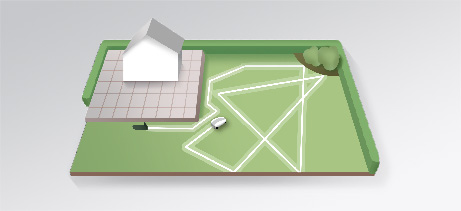
\includegraphics[scale=0.8]{figures/noLogiCut.jpg} 
\label{fig:randomcut}
\caption{Random cut system [source:Bosch]} 
\end{figure}

\noindent
When the battery is nearly discharged, the mower will follow the guard wire back to the base station for recharging.\\\\
\noindent
Parallel line mowers use a more intelligent control algorithm to optimize the mowing. After an initial learning run, following the guard wire around the lawn to be mowed, it will map the lawn, and cut in parallel lines, see \figref{fig:logicut}. The advantage of this strategy efficiency, as the lawn mower will not run over the same spots more than once. According to Bosch, a given lawn can be mowed up to 30\% faster with their Logicut system.
%% TODO: Insert source
 

\begin{figure}[H]
\centering
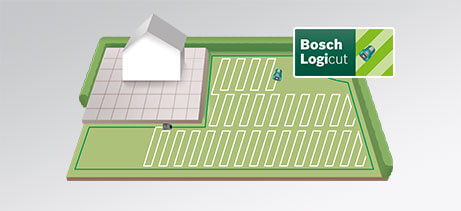
\includegraphics[scale=0.8]{figures/logicut.jpg} 
\label{fig:logicut}
\caption{Bosch Logicut system [source:Bosch]} 
\end{figure}

\noindent
Common for both systems is the guard wire, which has to be placed around the lawn and anywhere the lawn mower is not allowed to go, like flower beds, swimming pools, etc. \\\\
\noindent
This brings us to the problem with existing products.

\section{Problems with existing robotic lawn mowers}
All commercially available robotic lawn mowers requires a guard wire placed around the lawn. This can either be placed at the surface, and be held in place by pegs, or dug down below the surface. The guard wire must be routed around flower beds, etc. as well, see \figref{fig:robomow}

 
\begin{figure}[H]
\centering
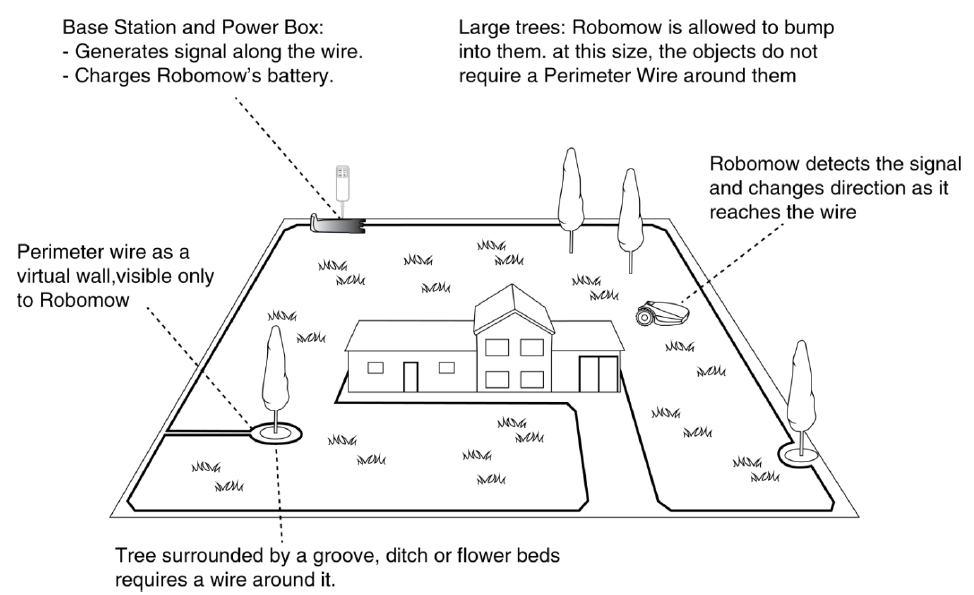
\includegraphics[scale=0.6]{figures/robomow.png} 
\label{fig:robomow}
\caption{Guard wire installation [source:Robomow]} 
\end{figure}
\noindent

The use of the guard wire for guiding the mower back to the charging station presents another potential problem: in a garden with many restricted areas, the guard wire could get very long. This could therefore make the journey home long, compared to a more direct route. This again uses more battery power, that instead could have been used for actually mowing the lawn.\\\\
\noindent
This will be the motivation for the project: to avoid the work routing a wire around the garden, and as a bonus get more work done on a battery charge, by not wasting power following the wire home.\\\\
\noindent
Then, the question is: What other solutions could be use to get the lawn mower to go where it has to go? \\
One first step could be to keep track of where it is in real-time.
%-- Section : GoT introductory presentation --%
\section{The Games on Track (GoT) system}
We were provided with the \emph{Games on Track GT-Position} system as a start to be able to determine the lawn mower's position in space. 
% Add reference to GoT description

\begin{figure}[H]
\centering
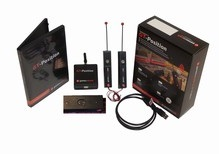
\includegraphics[scale=1.1]{figures/gotSystem.jpg} 
\label{fig:gotsystem}
\caption{Games on Track GT-Position package [source:Games\ on\ Track]} 
\end{figure}
\noindent

\noindent
It is composed of four different parts both hardware and software :
%% TODO : Add reference to http://www.gamesontrack.co.uk/pages/webside.asp?articleGuid=64556
\begin{itemize}
	\item A tracked module, which emits ultra-sound waves. It should be placed on the lawn mower itself while taking care, that the emitting cell is not obstructed by anything.
	\item Beacons or receivers, placed around the area the lawn mower will move in. Depending on the terrain, anywhere from 2 \todo{--Resolved-- is two enough? Answer: It is according to the GoT site (see reference in LaTeX comments)} to more than 20 of these can be used: the more is placed, the more accuracy can be obtained to fight against any ambient noise.
	\item The central system, which calculates the distance of the tracked module to each beacon, and transmits it to the computer via USB in regular intervals.
	\item The GoT software aggregates the received positions throughout time, and can be used to draw a map of the terrain (the lawn), and to determine the absolute position of the tracked module.
\end{itemize}

GoT was originally designed for train modelling, but it is easily adaptable for any use of position tracking and seems a good choice, at first, for our autonomous lawn mower.
But, why not use a satellite based positioning system ?

%-- Section : Satellite vs GoT --%
\section{Satellite based positioning systems vs GoT}
\todo{Wrong reasons for GPS vs GoT, elaborated below}
The reasons why satellite positioning system won't be used in our project are mainly related to accuracy over price ratios and to energy consumption.\todo{--To be reviewed again-- GPS uses very little power -> depending on the accuracy needed...}

\noindent
Indeed, these kinds of system like GPS or GLONASS would require a dedicated chip to put on the final system. The problem then would be the lack of precision. Although, there are some cheap standard GPS chips (around USD 10), these only reach around 1 meter of precision in the most ideal situations. % ref : www.gps.gov
On the other hand, the best GPS chips can achieve precisions up to a few millimeters when combined with different augmentation systems (algortihms for instance), but they end up being highly expensive (usually thousands of dollars). They are not generally intended for public use.
\todo{--To be reviewed again-- Only applies to cheap solutions, differential GPS can go to mm level, but is extremely expensive. This is what we are trying to replace with GoT, as it is a lot cheaper than diff-GPS} \\\\
%% TODO : Add reference to "A Review of GLONASS" Miller, 2000 & http://www.gps.gov/systems/gps/performance/accuracy/ 
\noindent
Moreover, if we add up the slow bit rates satellites can achieve, the signal amplifiers on the receiver, plus all the position calculations and possible augmentation systems, the total energy consumption would quickly rise,\todo{--To be reviewed again-- nope, it's just a radio receiver, uses almost no power} thus reducing the lawn mower autonomy, which is not desirable.\\
Indeed, the design of a product has no real value if no one is interested in using it. This is why choices made during this project have to be made in accordance with the final user's expectations.\\\\
\section{Potential consumer expectations}
Usually, we can think of a few priorities consumers will have when buying a product, whatever it is, and some more specific to technical products.\\
\noindent
Here for instance, the autonomy of the vehicle (both in energy and for the navigation), and the overall cost should be considered. The GoT system itself has a cost (USD 606.00 for a basic package) beyond anything a normal customer would probably pay for a lawn mower. But despite that, it appears, at first, to be a good solution for us in terms of accuracy and energy consumption compared to GPS-like systems which are even more expensive for the same accuracy. \todo{--Resolved-- insert price approximation here - not so true actually} \\\\
\noindent
These are the types of preliminary considerations that will influence this design process for an autonomous lawn mower.
% \section{Robotic Lawn Mowers}\label{roboMowers}
Several manufacturers of electrical gardening machines have started selling robotic lawn mowers in the recent years. In general they use one of these two strategies when cutting the lawn \todo{Source}:
%
\begin{itemize}
	\item Random direction mowers.
	\item Parallel line mowers.
\end{itemize}
%
Mowers utilizing the random direction strategy will drive in a straight line until a guard wire or an obstacle is detected. They will then turn in a random direction, and continue. See \figref{fig:randomcut}.

\begin{figure}[H]
\centering
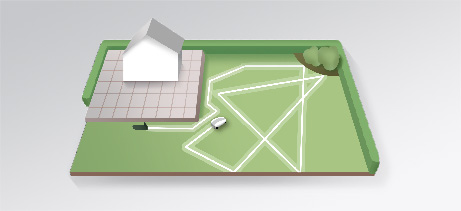
\includegraphics[scale=0.8]{figures/noLogiCut.jpg}
\caption{Random cut system \cite{Bosch}} 
\label{fig:randomcut}
\end{figure}
\noindent
When the battery is nearly discharged, the mower will follow the guard wire back to the base station to recharge.
%
Parallel line mowers utilize another control algorithm for mowing. After an initial learning run, following the guard wire around the lawn to be mowed, it will map the lawn, and cut in parallel lines, see \figref{fig:logicut}. The advantage of this strategy, is that the lawn mower will not run over the same spots more than once. According to Bosch, a given lawn can be mowed up to 30\% faster with their Logicut system \cite{Bosch}.

\begin{figure}[H]
\centering
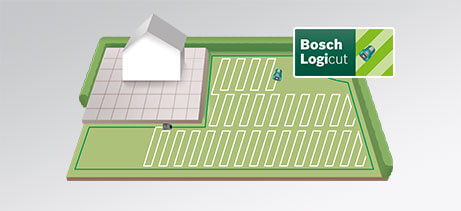
\includegraphics[scale=0.8]{figures/logicut.jpg} 
\caption{Bosch Logicut system \cite{Bosch}}
\label{fig:logicut}
\end{figure}
\noindent

Common for both systems is the guard wire, which has to be placed around the lawn and anywhere the lawn mower is not allowed to go, like flower beds, swimming pools, etc.
% \subsection{Existing Problems}
Some commercially available robotic lawn mowers require a guard wire placed around the lawn. It can either be installed at the surface, and be held in place by pegs, or dug down below the surface\todo{source?}. The guard wire must be routed around flower beds, bushes etc. as well, see \figref{fig:robomow}.\\\\
%
The use of the guard wire for guiding the mower back to the charging station presents another potential problem: in a garden with many restricted areas, the guard wire could get very long. Therefore the journey home could be longer, compared to a more direct route. This again uses more battery power, that could have been used for actually mowing the lawn instead.\\\\
%
This will be the motivation for the project: to avoid the work routing a wire around the garden, and as a bonus get more work done on a battery charge, by not wasting power following the wire home.\\\\

\begin{figure}[H]
\centering
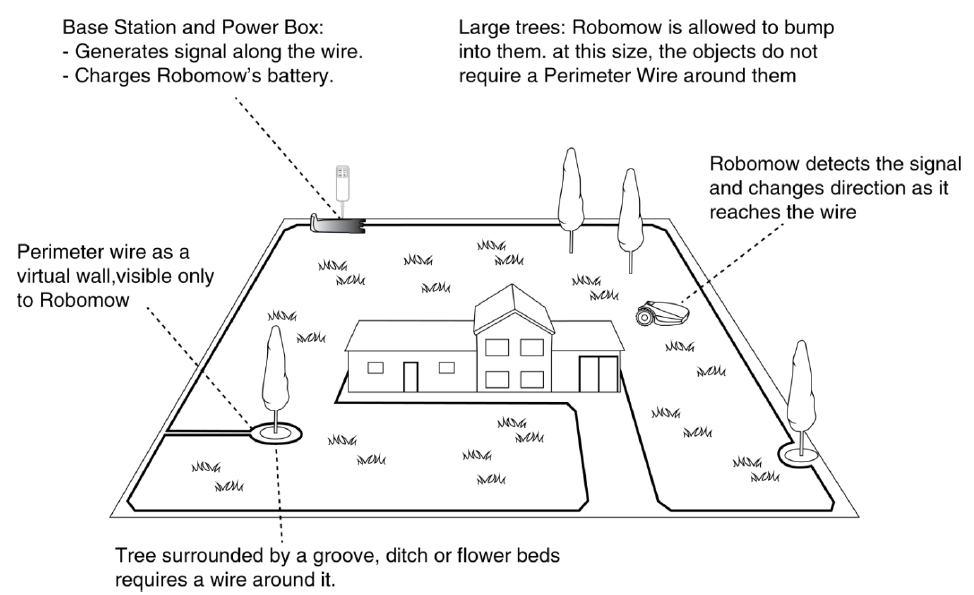
\includegraphics[scale=0.6]{figures/robomow.png} 
\caption{Guard wire installation [source:Robomow]}
\label{fig:robomow} 
\end{figure}
\noindent

Then, the next question is: what other solutions could be used to get the lawn mower to go where it has to go?
A solution of keeping track of the lawn mower's position in real-time is examined.
% %-- Section : GoT introductory presentation --%
\section{The Games on Track System}
One available system is the \emph{Games on Track GT-Position} system, referred to as GoT. The GoT would be able to determine the lawn mower's position in space, see \secref{sec:Vehicledescription}. It is composed of three different parts both hardware and software \cite{GoTWebsitePos}:

\begin{itemize}
	\item A tracked module, which emits ultra-sound and radio waves. It should be placed on the lawn mower itself.
	\item Towers which are tracking the tracked module placed on the vehicle are needed. These should be located around the area where the lawn mower will move. There should be at least 3 towers, depending on the terrain, and can be up to more than 20. The more towers, the more accuracy can be obtained to cancel out any ambient noise, and more space can be monitored.
	\item The master, connected to a computer, receives data from the towers and transmits it to computer through a USB in regular intervals. The distance of the tracked module is then calculated by the computer.
\end{itemize}

\begin{figure}[H]
\centering
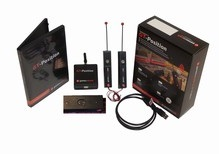
\includegraphics[scale=1.1]{figures/gotSystem.jpg} 
\caption{Games on Track GT-Position package [source:Games\ on\ Track]} 
\label{fig:GoTsystem}
\end{figure}
\noindent
%
The GoT software aggregates the received positions through time, and can be used to draw a map of the lawn, and to determine the absolute position of the tracked module.

GoT was originally designed for train modelling, but it is easily adaptable for any use of position tracking. In the following segment satellite based positioning systems are compared to the discussed GoT system.
% %-- Section : Satellite vs GoT --%
\section{Satellite based positioning systems vs GoT}
\todo{Wrong reasons for GPS vs GoT, elaborated below}
The reasons why satellite positioning system won't be used in our project are mainly related to accuracy-over-price ratios and to energy consumption.\todo{--To be reviewed again-- GPS uses very little power -> depending on the accuracy needed...}\\\\
Indeed, these kinds of system like GPS or GLONASS would require a dedicated chip to put on the final system. The problem then would be the lack of precision. Although, there are some cheap standard GPS chips (around USD 10), these only reach around 1 meter of precision in the most ideal situations \cite{GPSUSWebsiteAccuracy,Miller}. \\
On the other hand, the best GPS chips can achieve precisions up to a few millimeters \cite{GPSUSWebsiteAccuracy} when combined with different augmentation systems (algortihms for instance), but they end up being highly expensive (usually thousands of dollars). They are not generally intended for public use.
\todo{--To be reviewed again-- Only applies to cheap solutions, differential GPS can go to mm level, but is extremely expensive. This is what we are trying to replace with GoT, as it is a lot cheaper than diff-GPS} \\\\
%
Moreover, if we add up the slow bit rates satellites can achieve, the signal amplifiers on the receiver, plus all the position calculations and potential augmentation systems, the total energy consumption would quickly rise, \todo{--To be reviewed again-- nope, it's just a radio receiver, uses almost no power} thus reducing the lawn mower autonomy, which is not desirable.\\\\
%
Indeed, the design of a product has no real value if no one is interested in using it. This is why choices made during this project have to be made in accordance with the final user's expectations.
% \section{Consumer Expectations}
Usually, consumers have a few priorities when buying a product, whatever it is, and some more specific for technical products.\\
Here for instance, the autonomy of the vehicle (both in energy and for the navigation), and the overall cost should be considered. The GoT system itself has a cost (around \$ $600.00$ for the most basic package) beyond anything a normal customer would probably pay for a lawn mower. But despite that, it appears, at first, to be a good solution for a basic autonomous lawn mower in terms of accuracy and energy consumption compared to systems like GPS which are even more expensive for the same level of accuracy. \\\\
These are the types of preliminary considerations that will influence this design process for an autonomous lawn mower.

%% Chapter 2 %%
\chapter{Design Consideration}
\vspace{-5 mm}
In this chapter the system is designed with a top-down approach. First a use-case of the functionalities in the system is described, in order to give an overall view of what the system must be able to do. Hereafter, constraints set by time limitations as well as a focus on the main scope of the project, in regards to the prototype, is considered. Based on the use-case description and the prototype constraints the requirements for the systems prototype are listed.
\vspace{-4 mm}
\section{Use-case design}
To give an overall view of what the system should be able to do, a UML use-case diagram is used to consider and describe the main functionalities and operators in the system, see \figref{fig:usecase}.
\vspace{-3 mm}
 \begin{figure}[H]
	\centering
	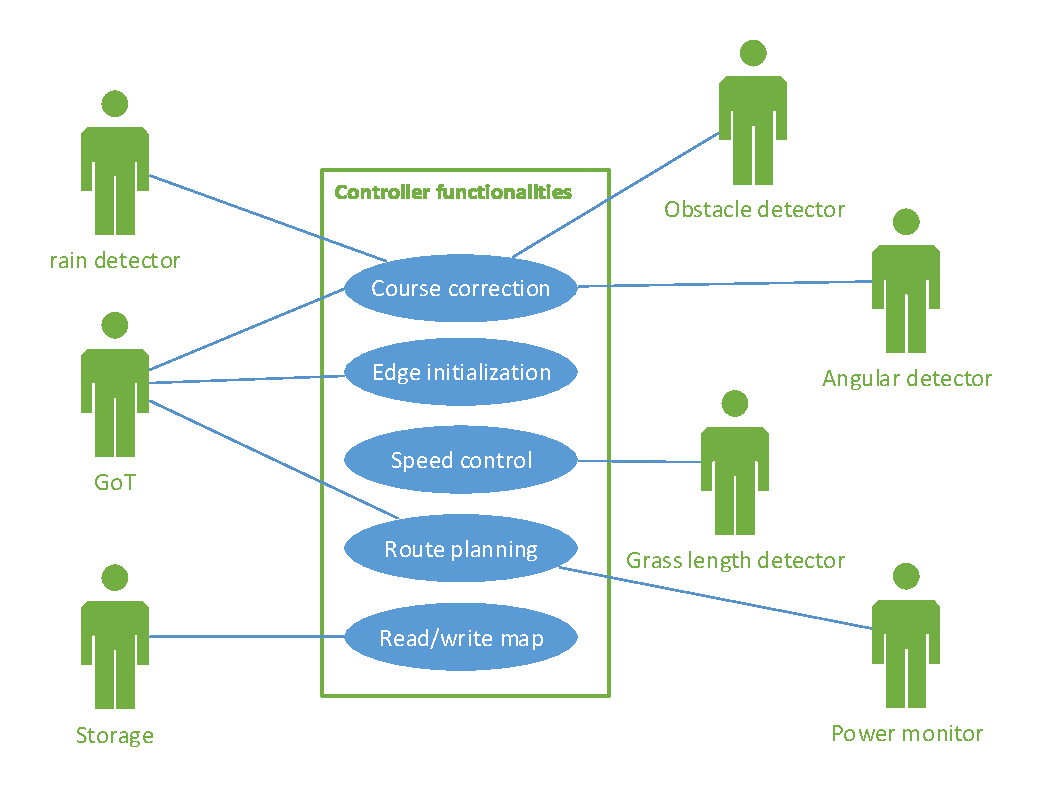
\includegraphics[scale=0.8]{figures/P5UseCase.pdf}
	\caption{Use-Case Diagram}
	\label{fig:usecase}
\end{figure}\vspace{-5mm}

\noindent
The main purpose of the system is to automatically navigate in a specific area which is confined by the \textit{edge initialization} functionality. This functionality handles the marking of the areas edges. The functionality is only used in the initialization process of the system. The concept is to only use the functionality after the GoT system has been positioned in the area. The consumer then takes the system around the edges of the grass, while the GoT system tracks its positions. It is therefore only necessary to reinitialize the system, if the GoT satellites has been moved. While the edge is being tracked, the \textit{edge initialization} uses the \textit{read/write map} functionality to store the information collected, in storage. \\\\ 
\noindent
The route in which the lawn mower is to navigate, in the specified area, is provided by the functionality \textit{route planning}. \textit{Route planning} uses the information, about the specific area, which is collected from the storage, to plan the most optimal route. Furthermore the \textit{route planning} needs information about the systems power level to insure the functionality is considering if the system needs charging and therefore have to return to the charging station at some point on the route.\\\\
\noindent
The \textit{read/write map} functionality as described earlier, handles the communication with storage. Hence it stores information, received from the \textit{edge initialization} and collects information from storage when the functionality \textit{route planning} needs it. \\\\
\noindent
To insure the system is moving with a desired speed (in a straight line and in a turn) or a speed which is fitted to the height of the grass, detected with the \textit{grass length detector}, a \textit{speed control} functionality is necessary in the system to control the motors. To insure the \textit{speed control} can deliver the desired speed an \textit{angular sensor} is utilized. \\\\
\noindent
The last functionality, \textit{course correction} is used when the system strays of the path calculated by \textit{route planning} or if the path gets blocked.
The obstacle which is blocking the route is detected by the sensor \textit{obstacle detector}. Furthermore the GoT system and the \textit{angular detector} will detect if the system is not on the desired path, or if the system starts to slip. Also, if it starts to rain, which is detected by the \textit{rain detector}, the system has to return to the charging station.
Finally, the \textit{course correction} sends the calculated data to the functionality \textit{speed control}. \\\\
\noindent
The overall functionalities of what the system must be able to do has been described. Now the different constraints on the system will be considered and the project prototype should be established.
\section{Prototype Constraints}\label{sec:PrototypeConstraints}
Before the prototype can be established, some considerations have to be made in respect to time limitations and the main scope of this semester. The aim of the project is to create a functional automated proof of concept lawn mower. The following section provides argumentation for eliminated functionalities from the use case \secref{sec:UseCase}.

\subsection{Grass Length Detection}
Detection of the grass length to control the velocity of the lawn mower thus ensuring an evenly cut lawn, is a submodule which can be added at any time. Since it is not fatal for a working system and might even be unnecessary depending on time between each mowing of the lawn, it is decided to exclude this functionality from the initial design.

\subsection{Humidity Sensor}
As the lawn mower is supposed to work outside, it is important to consider that the grass could be humid. Since it is difficult to cut wet grass, a humidity sensor could be used to warn the system of the humidity, thus the system could go back to the charging station. This submodule is not fatal for a functional prototype, so this type of sensor will not be included in the design.

\subsection{Obstacle Avoidance}
The lawn movers path might not always be clear, e.g. garden tools, tables or moving objects could be in the way. The vehicle should be aware of what is in front of it at any time, to correct its path and be able to get around the obstacle if necessary. To avoid this the sensor could be a pushing button to detect a solid object or an ultrasound detector if the object is fragile.
As the aim of the project is to control the path of the vehicle by using angular positioning sensors, a proximity sensor will not be included. Static objects could be registered on the map to avoid these issues.

Furthermore the edge mapping functionality will not be included in the project which instead will focus on a map predefined in the test room.

%\subsection{Power Monitoring}
%Power monitoring could be implemented by measuring the voltage across the batteries, to ensure that the lawn mower is not running out of power, and to ensure the vehicles calculated route passes the charging station before the power runs too low.
%This and the charging station will not be in the prototype, since it is beyond the scope of the project this semester and is not crucial for a working prototype.

\subsection{Blade Control \& Blade Monitor}
To get the blade to cut the grass evenly over the whole lawn, the blade control and monitor is needed to keep the blade at the same velocity.
The blade, and therefore the blade control and monitor, will not be in the prototype. This is because, the focus of the project is on the movement of the vehicle and the blade does not contribute to this and is therefore not relevant.

\subsection{Route Planning}
Route planning is a way to optimizing the lawn mowers time on the lawn, instead of the classic solution with a random cut system, describe in \secref{roboMowers}. The prototype will not have a algorithm calculating a route from the vehicle's position, the battery time and information received from the edge map. The route in which to follow is a predefined route made to illustrate and test the essential part of the prototype.

\subsection{Testing}
The testing will take place in Aalborg University Vicon Room, where the GoT system is installed, see \secref{GoTDescription}, is installed and calibrated with the appurtenant transmitter, which is mounted on the tracked vehicle during test.

A description of the system and arguments for eliminating functionalities from the initial design has been presented in the preceding segment. The prototype can now be established in regards to the equipment available and remaining functionalities.


% %% Part 2 %% %

\part{Design \& implementation}

% %% Part 3 %% %

\part{Test \& conclusion}

%% literaturliste og bilag %%
\bookmarksetup{startatroot}% this is it
\addtocontents{toc}{\bigskip}% perhaps as well
%\bibliography{setup/mybib}
%\label{bib:mybiblio}
 
 \newpage
 \fancyhead[RO]{\color{aaublue}\small Appendix \nouppercase\rightmark} %even page - chapter title
 \fancyhead[LE]{\color{aaublue}\small Appendix \nouppercase\rightmark} %uneven page - sectionhttps://88df6ea0630aed8027ff-0caf779119a6537399728d4d80523795.ssl.cf5.rackcdn.com/tcgyzshtzfpq/page/7cd587cdbc0ae962c2755c91cf17670aac438f1c.jpeg title
\fancyhead[RE,LO]{}
 \titleformat{\section}[hang]{\Large\bfseries}{\thesection\hsp\textcolor{aaublue}{|}\hsp}{0pt}{\Large\bfseries}

 \renewcommand{\thesection}{\Alph{section}}
 \setcounter{section}{0}

% %% appendix %% 
 
 \chapter*{Appendix}
 \addcontentsline{toc}{chapter}{Appendix}
	%\section{Figure Sample}

\begin{figure}[H]
	\caption{CAPTION\fxnote{Remember source}}
	\label{LABEL}
	\centering
	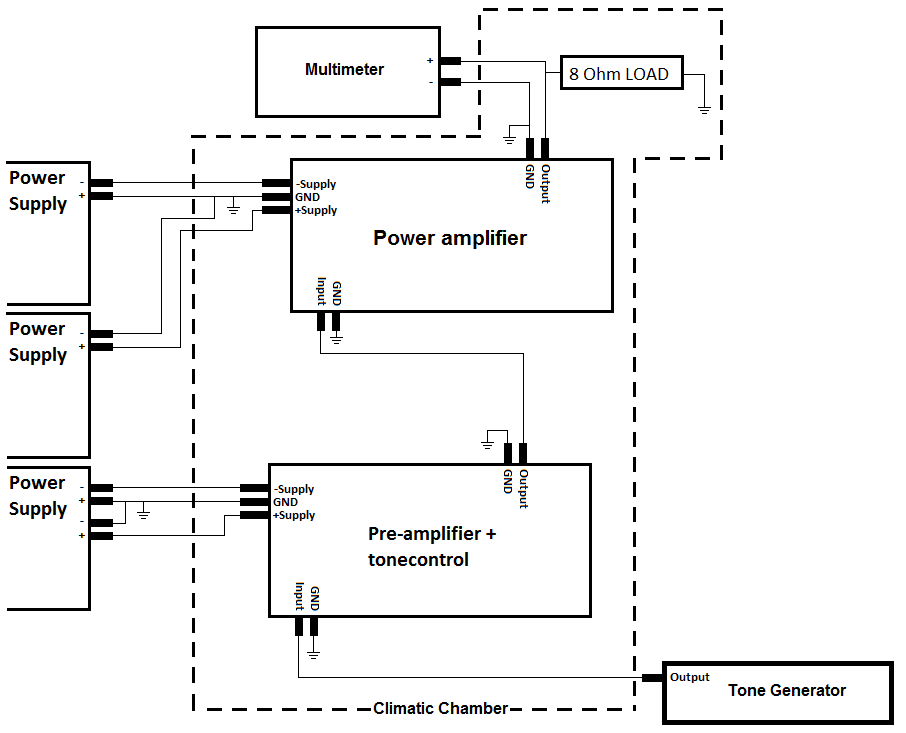
\includegraphics[scale=.6]{figures/filename}
	\flushleft
	\textit{SOURCE}
\end{figure}

%--------- NOTES ------------------------------------------------------
%Fxnotes wont compile properly inside the figure, only in the caption.
%Filetype ([...]{figures/filename.jpg}) can be specified but isn't needed.

\figref{LABEL} \Figref{LABEL}

%Do not use \vspace{length} or \hspace{length} or \noindent etc unless exceedingly necessary - LaTeX is a markup language, let it do its job.
\vspace{.5cm}
\noindent
%--------- BIBLIOGRAPHY REF EKSAMPLE -----------------------------------
This reference only represents this line since it is before the punctuation mark\cite{YDing}. This next reference however represents the entire section. That is all of the preceding sentences in the entire section. This is due to the fact that it is now after the punctuation mark in the end of the section (this is not used in the middle of a section!).\cite{YDing}
%>>>>>>>>>>>>>>>PLEASE ALSO READ THE NOTE IN bibliography/bibliography.bib<<<<<<<<<<<<<<<<<<
\pagebreak
	%\input{appendix/aTestTemplate.tex}
	%\section{Table Sample}

\begin{table}[H]
\caption{This Is a Table\label{LABEL}}
\begin{tabular}{|l|p{5cm}|l|l|l|}
  \hline %-----------------------------------------------------------------------------------
  \textbf{No.} &\textbf{Description} &\textbf{Min} &\textbf{Max} &\textbf{Requirements}    \\
  \hline %-----------------------------------------------------------------------------------
  1            & Some Text           & Some Text   & Some Text   & Some Text               \\
               &                     &             &             & Some More Text          \\
               &                     &             &             & Text Text               \\
               &                     &             &             & Text Text Text          \\
  \hline %-----------------------------------------------------------------------------------
  2            & Some Text           & Some Text   & Some Text   & Some Text               \\
  \hline %-----------------------------------------------------------------------------------
  3            & By specifying the
                 width of a column
                 (|p\{5cm\}|) the
                 cells in that column
                 will not exceed the
                 specified width but         %Extra hitespaces is used only for clarity
                 instead expand              %and will not affect the compiled output.
                 downward.
                                     & Some Text           & Some Text   & Some Text       \\
  \hline %-----------------------------------------------------------------------------------
  4            & Some Text           & Some Text   & Some Text   & Some Text               \\
  \hline %-----------------------------------------------------------------------------------
  \multicolumn{2}{|l|}{Some Text}    & \multicolumn{3}{l|}{Some Text}                      \\
  \hline %-----------------------------------------------------------------------------------
  \multicolumn{2}{|l|}{Text Text}    & \multicolumn{3}{l|}{Text = Text}                    \\
  \multicolumn{2}{|l|}{}             & \multicolumn{3}{l|}{Text = Text}                    \\
  \multicolumn{2}{|l|}{}             & \multicolumn{3}{l|}{Text = Text}                    \\
  \multicolumn{2}{|l|}{}             & \multicolumn{3}{l|}{Text = Text}                    \\
  \multicolumn{2}{|l|}{}             & \multicolumn{3}{l|}{Text = Text}                    \\
  \hline %-----------------------------------------------------------------------------------
  \multicolumn{2}{|l|}{Some Text}    & \multicolumn{3}{l|}{Teeeexxtt}                      \\
  \multicolumn{2}{|l|}{}             & \multicolumn{3}{l|}{\LaTeX}                         \\
  \hline %-----------------------------------------------------------------------------------
\end{tabular}
\end{table}

\tableref{LABEL} \Tableref{LABEL}

\pagebreak
	%\section{Equation Sample}

Ohms Law:
\begin{flalign}
  U &= I \times R \unit{\volt}
  \label{eq1}
\end{flalign}
%
Some explanation:
\begin{flalign}
  [Equation] &= [Number] \unit{Unit}
  \label{eq2}
\end{flalign}
%
Some explanation:
\begin{flalign}
  [Equation] &= [Number] \unit{Unit}
  \label{eq3}
\end{flalign}
%
Some explanation:
\begin{flalign}
  [Equation] &= [Number] \unit{Unit}
  \label{eq4}
\end{flalign}
%
Some explanation:
\begin{flalign}
  [Short Equation] &= [Number] \unit{Unit}
  \label{eq5}\\ %<-------------------------------------------------| Remember linebreak AFTER
  [Somewhat Longer Equation] &= [Number] \unit{Unit} %             | label when writing multiple
  \label{eq6}\\ %<-------------------------------------------------| equations.
  [Somewhat Quite a Lot Longer Equation] &= [Number] \unit{Unit}
  \label{eq7}
\end{flalign}
%
%
\eqref{eq1}\\
%
\eqrefTwo{eq1}{eq2}\\
%
\eqrefThree{eq1}{eq2}{eq3}\\
%
\eqrefFour{eq1}{eq2}{eq3}{eq4}\\
%
\eqrefFive{eq1}{eq2}{eq3}{eq4}{eq5}\\
%
\eqrefSix{eq1}{eq2}{eq3}{eq4}{eq5}{eq6}\\
%
\eqrefSeven{eq1}{eq2}{eq3}{eq4}{eq5}{eq6}{eq7}\\
%
\Eqref{eq1}\\
%
\EqrefTwo{eq1}{eq2}\\
%
\EqrefThree{eq1}{eq2}{eq3}\\
%
\EqrefFour{eq1}{eq2}{eq3}{eq4}\\
%
\EqrefFive{eq1}{eq2}{eq3}{eq4}{eq5}\\
%
\EqrefSix{eq1}{eq2}{eq3}{eq4}{eq5}{eq6}\\
%
\EqrefSeven{eq1}{eq2}{eq3}{eq4}{eq5}{eq6}{eq7}
%
\pagebreak
	\section{The Games on Track GT-position system}
The Games on Track GT-Position system, shortened GoT, is a GPS system which uses radio-waves and ultrasound to locate the object. The system is build up by three hardware components, the transmitter, receiver and master. 

\subsubsection{Transmitter}
The transmitter component is placed on the object, which needs to be located. To indicate the objects position, the transmitters emits out ultrasound waves to indicate where it and the object is positioned. The transmitter component runs on 2 AA-batteries and therefore does not need an external power-source. 

\subsubsection{Receiver}
\todo{What kind of "radio waves" does the receiver transmit data to the master?}
The receiver component is placed around the area where the object, with the transmitter, has to be located. The receivers assignment is to search for the ultrasound waves, which the transmitter is emitting. The ultrasound waves received by the receivers, provides information containing the distance between the specific receiver to the transmitter located on the object. To be able to calculate the exact position of the transmitter and the object, a minimum of three receivers is necessary. however, more receivers can be added to the system for more reliability and the ability to cover a larger area. For the receivers to work at a high efficiency, they should be placed 1 to 2 meters apart and not on a single line. But if receivers shall cover a bigger area, they can be placed up to a distance of 5 meters between them, however, this would affect the measurement and thereby make it less reliable. Each receiver have a maximum range of 8 meters and as seen on \figref{receiverSetup}, the three receivers should be placed in each others reach. The receivers needs between 14 to 20 volt DC. Thus, making the receivers able to be powered through a computer charger if necessary.

\begin{figure}[H]
	\centering
	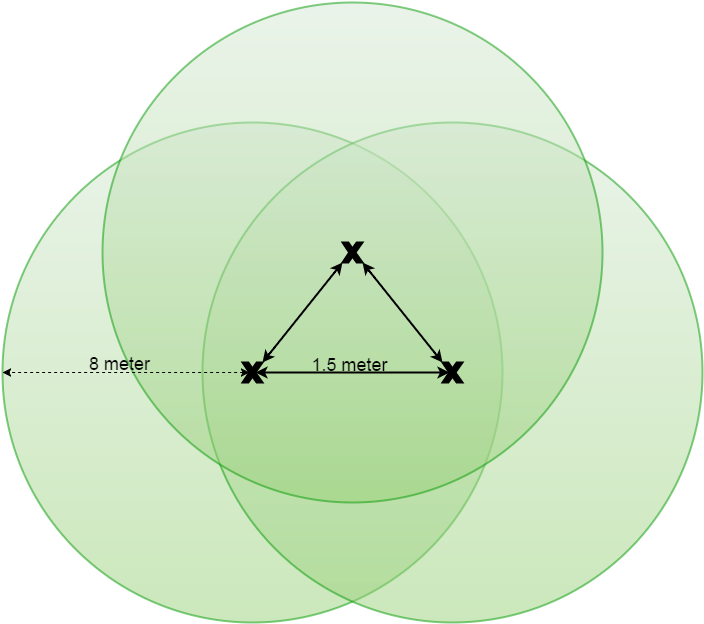
\includegraphics[scale=0.5]{figures/ReceiverSetup.png}
	\caption{Example on a standard setup for the receivers (increase size of text in figure)}
	\label{receiverSetup}
\end{figure}

\subsubsection{Master}
The master is a receiver which should be connected to a computer. The masters assignment is to receive the data transmitted from the individual receivers and send it directly to the connected computer. The master is powered through a USB cable, between the master and the computer.
\subsubsection{Computer}

The program on the computer, which handles the information received from the master, uses the data to calculate the position of the transmitter. This is done with a method call Trilateration. Trilateration is a way of calculating a position, in a three-dimensional space, from three distances (from known locations), with the help of spheres, circles and triangles. Therefore it is necessary for the system to have atleast three receivers, as mentioned earlier. With additional receivers a check up can be performed to ensure the position of the transmitter is correct.\\\\

If the receivers have been moved, it is necessary to calibrate the system. This is done with a calibration triangle. The calibration triangle is three markings on the surface, that will be setup to be the zero surface for the Z-axis. One of the points on the calibration triangle is made the origin (0,0,0) of the coordinate system. Another point on the triangle will then be call (X,0,0), in which the line between the first point and the second point will become the X-axis. The last point will be call (X,Y,0) and will determine in which way the positive Y-axis will go. The surface which the calibration triangle is creating, will be the zero surface for the Z-axis, and is horizontal. The distance between the three points is measured and put into the software. Thereafter, with using the transmitter, are the position of the receivers calculated.  The transmitter is first placed in the first point (0,0,0), there next the second point (X,0,0) and then in the last point (X,Y,0). At each point the distance to the receivers is measured. Out from this data, about the placement of the points and their distance to the receivers, the software can calculate the position of each receiver, with the help of trilateration. \\\\

\todo{How should the recievers be placed? how far can they reach, picture?}

\todo{How do you calibrate, do you move the transmitter around?? but that in the text}

\todo{mergeconflict which needs to be addressed}

The program on the computer, which handles the information received from the master, uses the data to calculate the position of the transmitter. This is done with a method call Trilateration. Trilateration is a way of calculating a position, in a three-dimensional space, from three distances (from known locations), with the help of spheres, circles and triangles. Therefore it is necessary for the system to have atleast three receivers, as mentioned earlier.  With additional receivers a check up can be performed to ensure the position of the transmitter is correct. Trilateration does not work, if the three know points is on a single line and therefore shall the receivers be placed in a triangle.\\\\
\noindent
If the receivers have been moved, it is necessary to calibrate the system. This is done with a calibration triangle. The calibration triangle is made of three points on a flat surface and have a distance of 40 to 200 centimeters between them. One of the points on the calibration triangle is made the origin (0,0,0) of the new coordinate system. Another point on the triangle will then be call (X,0,0), in which the line between the first point and the second point will become the X-axis. The last point will be call (X,Y,0) and will determine in which way the positive Y-axis will go. The surface which the calibration triangle is placed on, will be the XY-plan, where Z will go positiv in the direction of the receivers. The distance between the three points is measured and put into the program. Thereafter, the transmitter placed in the three point, with (0,0,0) first and (X,Y,0) last. When the transmitter is placed in a point, the receivers measure the distance between them and the transmitter. From the data, the program can calculate the position of each receiver, with the help of trilateration. \\\\

% \input{appendix/koleplade.tex} %skal være input for at undgå den skifter 
  
  \pagebreak
\section{Motor Tests}
\nopagebreak
\subsection{Armature Resistance} %\label{put a label here and uncomment}
\textbf{Name: Group 510}\\
\textbf{Date: 30/09 - 2015}

\subsubsection{Purpose}
The purpose of the test is to measure the armature resistance $R_a$ of the motor.

\subsubsection{Setup}
\begin{figure}[H]
  \centering
	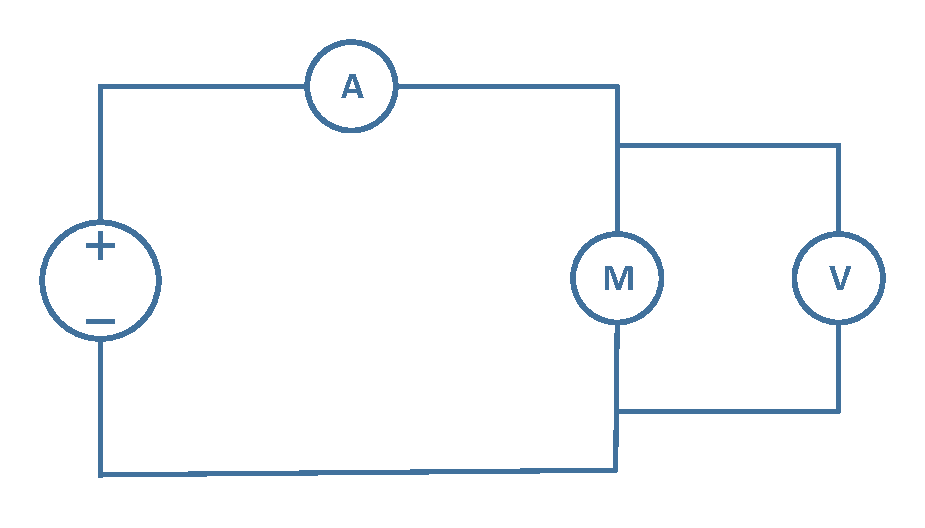
\includegraphics[scale=0.5]{figures/MotorTest1.pdf}
	\caption{Setup diagram}
\end{figure}

\subsubsection{List of Equipment}
\begin{table}[H]
\begin{tabular}{|l|l|p{4cm}|}
\hline%------------------------------------------------------------------------------------
  \textbf{Instrument}                        &  \textbf{AAU-no.}  &  \textbf{Type}       \\
\hline%------------------------------------------------------------------------------------
  Multimeter 1                               &  60764             &  Fluke 189 True RMS  \\
\hline%------------------------------------------------------------------------------------
  Multimeter 2                   		         &  60769             &  Fluke 189 True RMS  \\
\hline%------------------------------------------------------------------------------------
  Power Supply \small{(0 - 32 V) (0 - 10 A)} &  77076             &  Ea - ps 7032 - 100  \\
\hline%------------------------------------------------------------------------------------
  Clamp for fixing the motor                 &  03039             &                      \\
\hline%------------------------------------------------------------------------------------
\end{tabular}
\end{table}

\subsubsection{Procedure}

\begin{enumerate}
  \item Turn on the two multimeters and choose Voltage and Ampere settings respectively.
  \item Fix the motor shaft so it can not turn.
  \item Choose the first current value ($0,5$ A) on the current limiting of the power supply.
  \item Turn on the power supply and adjust the current limiting in accordance with the ampere meter.
  \item Read the voltage supplied to the motor from the volt meter.
  \item Repeat the three previous steps for each measurement in $0,5$ A increments up to $5$ A.
  \item Switch the poles of the power supply and repeat the measurements in the negative direction.
\end{enumerate}

\subsubsection{Results}

\begin{table}[H]
\begin{tabular}{|l|l|l| l|l|}
\cline{1-2}\cline{4-5}%-----------------------             ----------------------------------------------
  \textbf{Input (A)}   & \textbf{Output (V)} &\phantom{hey}& \textbf{Input (A)}   & \textbf{Output (V)}\\
\cline{1-2}\cline{4-5}%-----------------------             ----------------------------------------------
  $-5,0$               &            $-0,71$  &             & $0,5$                & $0,16$             \\
\cline{1-2}\cline{4-5}%-----------------------             ----------------------------------------------
  $-4,5$               &            $-0,65$  &             & $1,0$                & $0,34$             \\
\cline{1-2}\cline{4-5}%-----------------------             ----------------------------------------------
  $-4,0$               &            $-0,59$  &             & $1,5$                & $0,53$             \\
\cline{1-2}\cline{4-5}%-----------------------             ----------------------------------------------
  $-3,5$               &            $-0,54$  &             & $2,0$                & $0,62$             \\
\cline{1-2}\cline{4-5}%-----------------------             ----------------------------------------------
  $-3,0$               &            $-0,43$  &             & $2,5$                & $0,64$             \\
\cline{1-2}\cline{4-5}%-----------------------             ----------------------------------------------
  $-2,5$               &            $-0,36$  &             & $3,0$                & $0,75$             \\
\cline{1-2}\cline{4-5}%-----------------------             ----------------------------------------------
  $-2,0$               &            $-0,27$  &             & $3,5$                & $0,78$             \\
\cline{1-2}\cline{4-5}%-----------------------             ----------------------------------------------
  $-1,5$               &            $-0,20$  &             & $4,0$                & $0,80$             \\
\cline{1-2}\cline{4-5}%-----------------------             ----------------------------------------------
  $-1,0$               &            $-0,14$  &             & $4,5$                & $0,83$             \\
\cline{1-2}\cline{4-5}%-----------------------             ----------------------------------------------
  $-0,5$               &            $-0,07$  &             & $5,0$                & $0,88$             \\
\cline{1-2}\cline{4-5}%-----------------------             ----------------------------------------------
\end{tabular}
\end{table}

\begin{figure}[H]
  \centering
 	%Trim margins @:   left        bottom       right       top
 	\adjustbox{ trim = {.15\width} {.30\height} {.15\width} {.30\height}, clip }
  {
    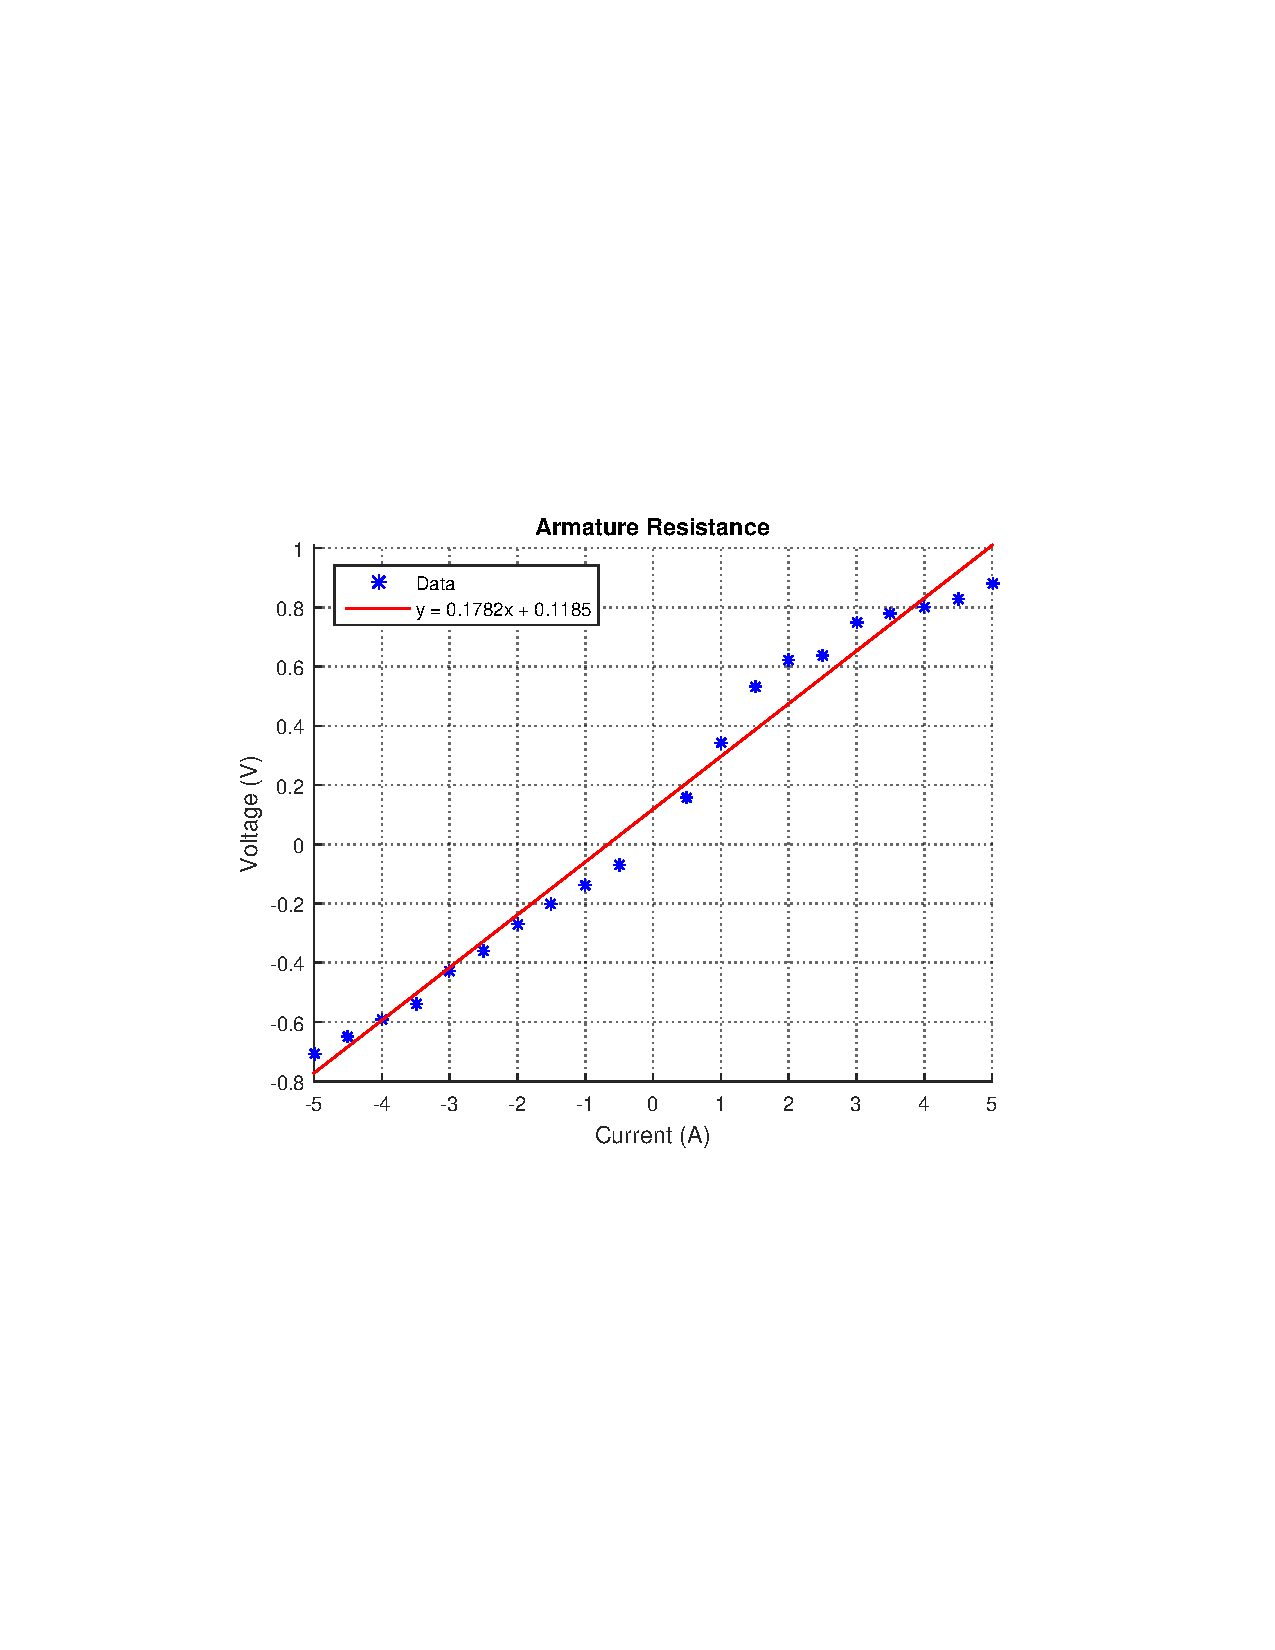
\includegraphics[width=\textwidth]{figures/armatureResistance.pdf}
  }
  \caption{A plot of a measured armature resistance, with a red line indicating the an average value.}
  \label{armatureResistance}
\end{figure}

During these measurements the motor is in steady state. This is necessary for the inductor in the armature coil to act as a short circuit, which allows easy calculation of the armature resistance. In steady state we get:

\begin{flalign}
  \eq{R_a} {\frac{U_a}{I_a}} \unit{\Omega}\nonumber
\end{flalign}
\hspace{6mm} Where:\\
\begin{tabular}{p{1cm}lll}
  & \si{I_a} & is the armature current    &\unitWh{A}    \\
  & \si{U_a} & is the armature voltage    &\unitWh{V}    \\
  & \si{R_a} & is the armature resistance &\unitWh{\Omega}  \\
\end{tabular}

As seen on the data plot in \figref{armatureResistance} the result is a relatively linear function. The armature resistance is approximated directly as the slope of the least square line: \todo{is it not invers?}
\begin{flalign}
  \eq{R_a}{0,178}\ \si{\Omega}&\nonumber
\end{flalign}
  \pagebreak
\subsection{Armature Inductance}%\label{put a label here and uncomment}
\textbf{Name: Group 510}\\
\textbf{Date: 30/09 - 2015}

\subsubsection{Purpose}
The purpose of the test is to determine the Armature inductance \si{L_a} of the motor.

\subsubsection{Setup}
\begin{figure}[H]
  \centering
	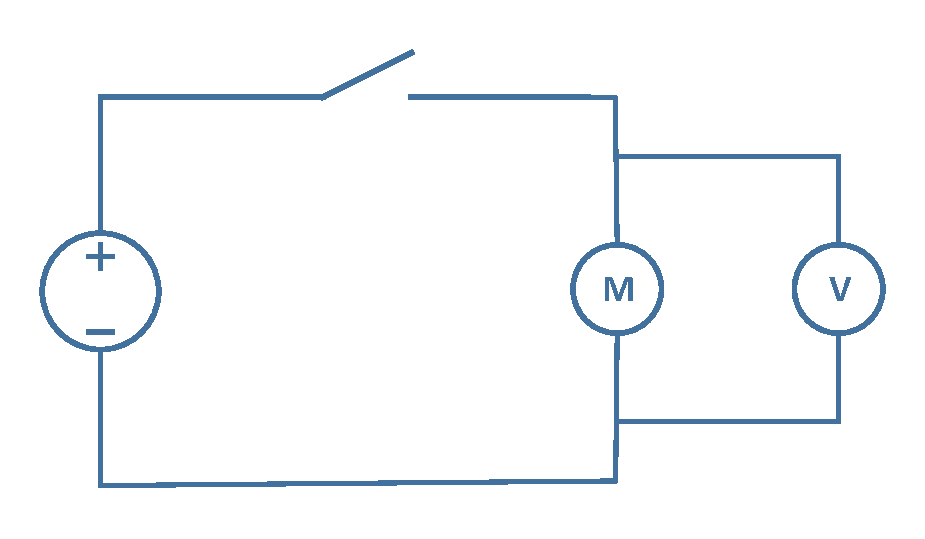
\includegraphics[scale=0.5]{figures/MotorTest2.pdf}
	\caption{Setup diagram}
\end{figure}

\subsubsection{List of Equipment}

\begin{table}[H]
\begin{tabular}{|l|l|p{4cm}|}
\hline%--------------------------------------------------------------------------------
  \textbf{Instrument}                    &  \textbf{AAU-no.}  &  \textbf{Type}       \\
\hline%--------------------------------------------------------------------------------
  Power Supply ($0 - 32$ V) ($0 - 10$ A) &  77076             &  Ea - ps 7032 - 100  \\
\hline%--------------------------------------------------------------------------------
  AC/DC Current Clamp (Output: 100 mV/A) &  78550             &  FLUKE i30s          \\
\hline%--------------------------------------------------------------------------------
  Oscilloscope                           &  64672             &  Agilent DSO6034A    \\
\hline%--------------------------------------------------------------------------------
  Clamp for fixing the motor             &  03039             &                      \\
\hline%--------------------------------------------------------------------------------
\end{tabular}
\end{table}

\subsubsection{Procedure}

\begin{enumerate}
  \item Fix the motor shaft so it can not turn.
  \item Start with the power supply disconnected and turn on the oscilloscope.
  \item On the oscilloscope press the "trigger mode"-key choose the "normal"-option and push the "single"-key.
  \item To prevent false triggering on the oscilloscope, set the trigger value to $113$ mV.
  \item To supply the motor a pulse of $5$ V, adjust the power supply to $5$ V and connect it.
  \item Connect a USB-drive to the oscilloscope and press the save key to extract the data.
\end{enumerate}

\subsubsection{Results}

\begin{figure}[H]
  \centering
 	%Trim margins @:   left        bottom       right       top
 	\adjustbox{ trim = {.15\width} {.30\height} {.15\width} {.30\height}, clip }
  {
    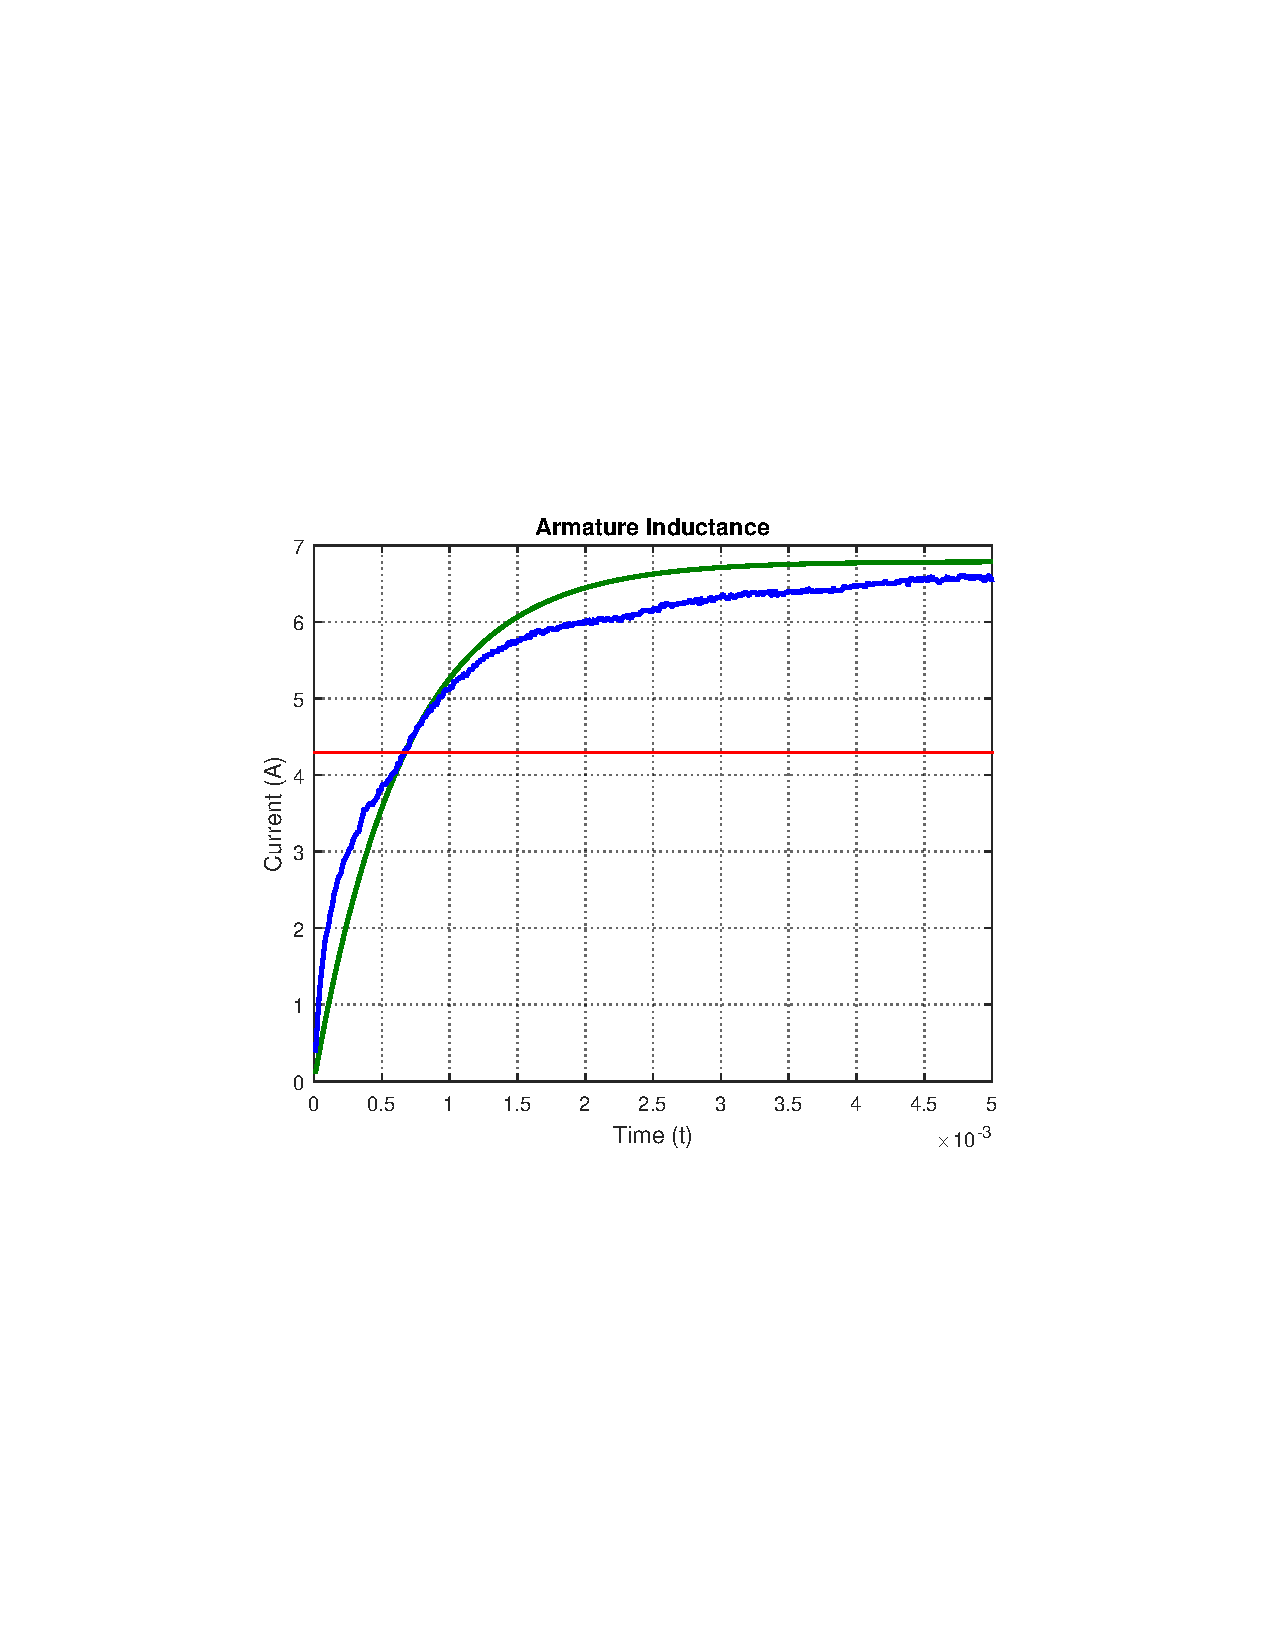
\includegraphics[width=\textwidth]{figures/armatureInductance.pdf}
  }
	\caption{A plot of a current step response of the motor, where the blue line is data, the green line is the ideal step response and the red line is the time constant}
	\label{armatureInductance}
\end{figure}

The armature inductance, \si{L_a}, is calculated from the time constant given by:
\begin{flalign}
  \eq{\tau} {\frac{L_a}{R_a}}\unit{s}\nonumber
\end{flalign}
\hspace{6mm} Where:\\
\begin{tabular}{p{1cm}ll}
  & \si{\tau} & is the time constant \unit{s}       \\
  & \si{L_a}  & is the armature inductance \unit{H} \\
  & \si{R_a}  & is the armature resistance \unit{\Omega} \\
\end{tabular}

\si{R_a} is know from the previous test, \textit{Armature Resistance}, where it was found to \si{0,178 \Omega}. $\tau$ is the time at which the current reaches \si{63,2\%} of the value at steady state. This value of $\tau$ is found by use of \figref{armatureInductance} and located in the data set:
%
\begin{flalign}
  \eq{\tau}{0,67 \cdot 10^{-3}}\unit{s}\nonumber
\end{flalign}
%
From this we get the armature inductance:
%
\begin{flalign}
  \eq{L_a}{\tau \cdot R_a}\unit{H}\nonumber\\
  \eq{L_a} {0,67 \cdot 10^{-3} \cdot 0,178}\unit{H}\nonumber\\
  \eq{L_a}{119,26}\unit{\mu H}\nonumber
\end{flalign}
  \pagebreak
\subsection{Tachometer Constant} %\label{put a label here and uncomment}
\textbf{Name: Group 510}\\
\textbf{Date: 30/09 - 2015}

\subsubsection{Purpose}
The purpose of the test is to measure verify that tachometer constant (in V) is 0,030 multiplied by the motor velocity in radians per second.

\subsubsection{Setup}
\begin{figure}[H]
  \centering
	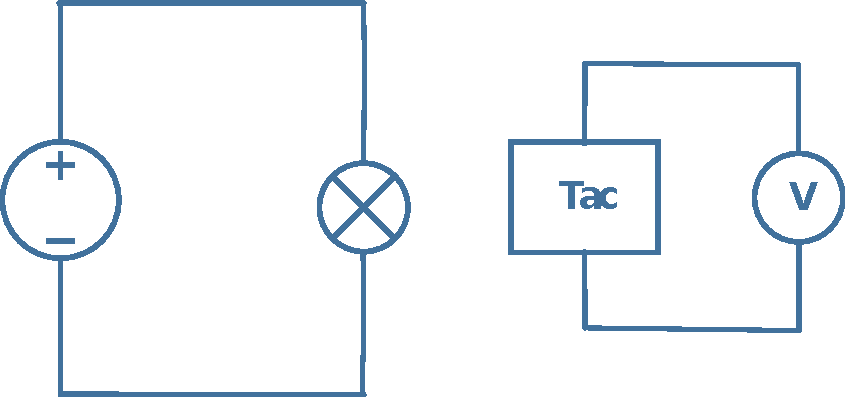
\includegraphics[scale=0.5]{figures/MotorTest3.pdf}
	\caption{Setup Diagram}
	\flushleft
\end{figure}

\subsubsection{List of Equipment}

\begin{table}[H]
\begin{tabular}{|l|l|p{4cm}|}
\hline%--------------------------------------------------------------------------------
  \textbf{Instrument}                    &  \textbf{AAU-no.}  &  \textbf{Type}       \\
\hline%--------------------------------------------------------------------------------
  Power Supply ($0 - 32$ V) ($0 - 10$ A) &  77076             &  Ea - ps 7032 - 100  \\
\hline%--------------------------------------------------------------------------------
  Multimeter                             &  60764             &  Fluke 189 True RMS  \\
\hline%--------------------------------------------------------------------------------
  Optical tachometer                     &  08246             &  Shimpo DT-205       \\
\hline%--------------------------------------------------------------------------------
\end{tabular}
\end{table}

\subsubsection{Procedure}

\begin{enumerate}
  \item Adjust voltage of power supply till the multimeter reaches $6$ V over the tachometer.
  \item Measure the RPM with the Optical tachometer.
\end{enumerate}

\subsubsection{Results}
The tachometer measured 1933 RPM at 6 V, which is used to verify a tachometer constant of \SI{0,03}:
%
\begin{flalign}
 \frac{1933}{60} \cdot 2 \cdot \pi \cdot \num{0,03} &= \num{6,07} \approx 6 \unit{V}
  \label{eqTachometerConstant}
\end{flalign}
  \subsection{Generator Constant} %\label{put a label here and uncomment}
\textbf{Name: Group 510}\\
\textbf{Date: 30/09 - 2015}

\subsubsection{Purpose}
The purpose of the test is to find the generator constant $K_e$ by measuring the motor voltages, currents and velocities, in several steady states.

\subsubsection{Setup}
\begin{figure}[H]
  \centering
	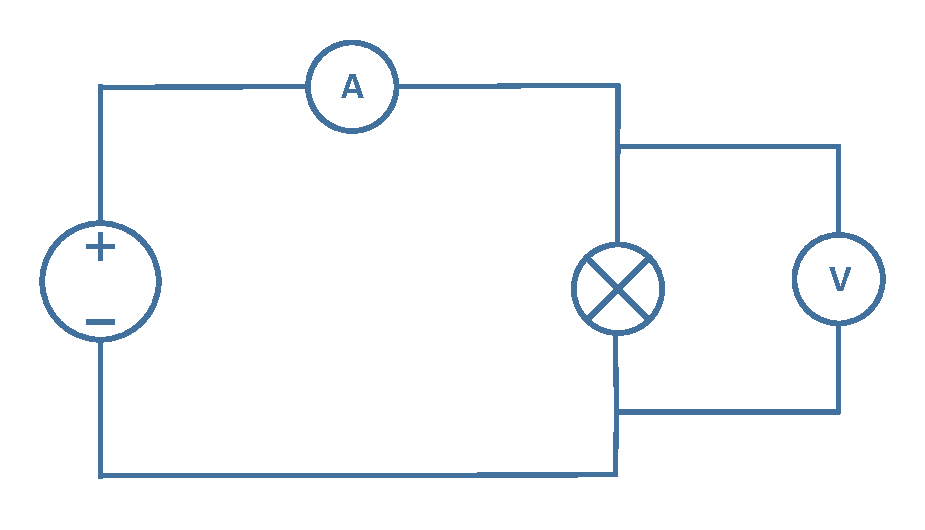
\includegraphics[scale=0.5]{figures/MotorTest4.pdf}
	\caption{Use-Case Diagram}
\end{figure}

\subsubsection{List of Equipment}

\begin{table}[H]
\begin{tabular}{|l|l|p{4cm}|}
\hline%------------------------------------------------------------------------------------
  \textbf{Instrument}                        &  \textbf{AAU-no.}  &  \textbf{Type}       \\
\hline%------------------------------------------------------------------------------------
  Multimeter 1                               &  60764             &  Fluke 189 True RMS  \\
\hline%------------------------------------------------------------------------------------
  Multimeter 2                   		         &  60769             &  Fluke 189 True RMS  \\
\hline%------------------------------------------------------------------------------------
  Power Supply ($0 - 32$ V) ($0 - 10$ A)     &  77076             &  Ea - ps 7032 - 100  \\
\hline%------------------------------------------------------------------------------------
  Optical tachometer                         &  08246             &  Shimpo DT-205       \\
\hline%------------------------------------------------------------------------------------
\end{tabular}
\end{table}

\subsubsection{Procedure}

\begin{enumerate}
  \item Turn on the two multimeters and put them in ampere and voltage mode respectively.
  \item Apply $1$ V by use of the voltage mode multimeter
  \item Read out the current value from the ampere mode multimeter
  \item Read out RPM of the motor using the optical tachometer.
  \item Repeat the past $3$ steps up to $7$ V in $1$ V increments.
\end{enumerate}

\subsubsection{Results}

\begin{table}[H]
\begin{tabular}{|l|l|l|l|}
\hline%----------------------------------------------------------------
  \textbf{Input (V)}  & \textbf{Output (A)} & \textbf{Output (RPM)} & \textbf{Generator constant} \\
\hline%----------------------------------------------------------------
  $1$                 &            $1.7$  &  $3684$ & $0.00181$                 \\
\hline%----------------------------------------------------------------
  $2$                 &            $2.2$  &  $8063$ & $0.00191$                 \\
\hline%----------------------------------------------------------------
  $3$                 &            $2.6$  &  $12021$ & $0.00202$                \\
\hline%----------------------------------------------------------------
  $4$                 &            $3.3$  &  $16746$ & $0.00195$                \\
\hline%----------------------------------------------------------------
  $5$                 &            $4.1$  &  $21966$ & $0.00186$                \\
\hline%----------------------------------------------------------------
  $6$                 &            $4.8$  &  $26420$ & $0.00186$                \\
\hline%----------------------------------------------------------------
  $7$                 &            $5.6$  &  $31447$ & $0.00182$                \\
\hline%----------------------------------------------------------------
\end{tabular}
\end{table}

The equation for the generator constant is $K_e = \frac{U_a - R_a I_a}{\omega}$. The generator constants for each measurement is not equal, but with a small margin in difference. The average generator constant is $0.00189$.
  \pagebreak
\subsection{Motor Constant} %\label{put a label here and uncomment}
\textbf{Name: Group 510}\\
\textbf{Date: 30/09 - 2015}

\subsubsection{Purpose}
The purpose of this of this test is to measure the motor constant \si{K_t}.

\subsubsection{Setup}
\begin{figure}[H]
  \centering
	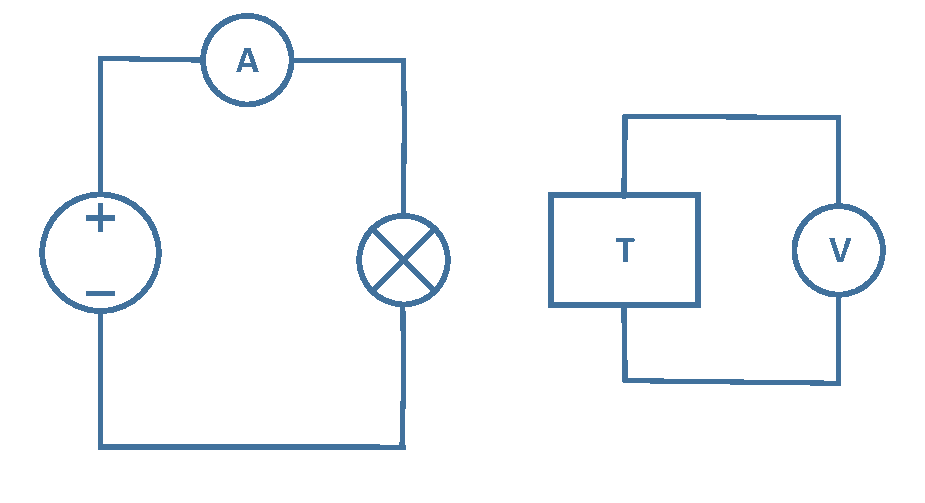
\includegraphics[scale=0.5]{figures/MotorTest5.pdf}
	\caption{Setup diagram}
\end{figure}

\subsubsection{List of Equipment}

\begin{table}[H]
\begin{tabular}{|l|l|p{4cm}|}
\hline%------------------------------------------------------------------------------------
  \textbf{Instrument}                        &  \textbf{AAU-no.}  &  \textbf{Type}       \\
\hline%------------------------------------------------------------------------------------
  Multimeter 1                               &  60764             &  Fluke 189 True RMS  \\
\hline%------------------------------------------------------------------------------------
  Multimeter 2                   		         &  60769             &  Fluke 189 True RMS  \\
\hline%------------------------------------------------------------------------------------
  Power Supply ($0 - 32$ V) ($0 - 10$ A)     &  77076             &  Ea - ps 7032 - 100  \\
\hline%------------------------------------------------------------------------------------
  Torque sensor                              &  08772             &  Icom                \\
\hline%------------------------------------------------------------------------------------
\end{tabular}
\end{table}

\subsubsection{Procedure}

\begin{enumerate}
  \item Connect the motor shaft to the torque sensor.
  \item Turn on the two multimeter in current and voltage mode respectively.
  \item Start by setting the power supply at 1 A current limiting.
  \item Turn on the supply and note the voltage across the torque sensor.
  \item Repeat the previous two steps up to 10 A with 1 A increments.
\end{enumerate}

\subsubsection{Results}

\begin{table}[H]
\begin{tabular}{|l|l|l|}
\hline%-----------------------------------------
  \textbf{Input (A)}  & \textbf{Output (V)}  \\
\hline%-----------------------------------------
  $1$                 &            0,107    \\
\hline%-----------------------------------------
  $2$                 &            0,113    \\
\hline%-----------------------------------------
  $3$                 &            0,118    \\
\hline%-----------------------------------------
  $4$                 &            0,122    \\
\hline%-----------------------------------------
  $5$                 &            0,131    \\
\hline%-----------------------------------------
  $6$                 &            0,142    \\
\hline%-----------------------------------------
  $7$                 &            0,149    \\
\hline%-----------------------------------------
  $8$                 &            0,158    \\
\hline%-----------------------------------------
  $9$                 &            0,169    \\
\hline%-----------------------------------------
  $10$                &            0,180    \\
\hline%-----------------------------------------
\end{tabular}
\end{table}

\begin{figure}[H]
  \centering
 	%Trim margins @:   left        bottom       right       top
 	\adjustbox{ trim = {.15\width} {.30\height} {.15\width} {.30\height}, clip }
  {
    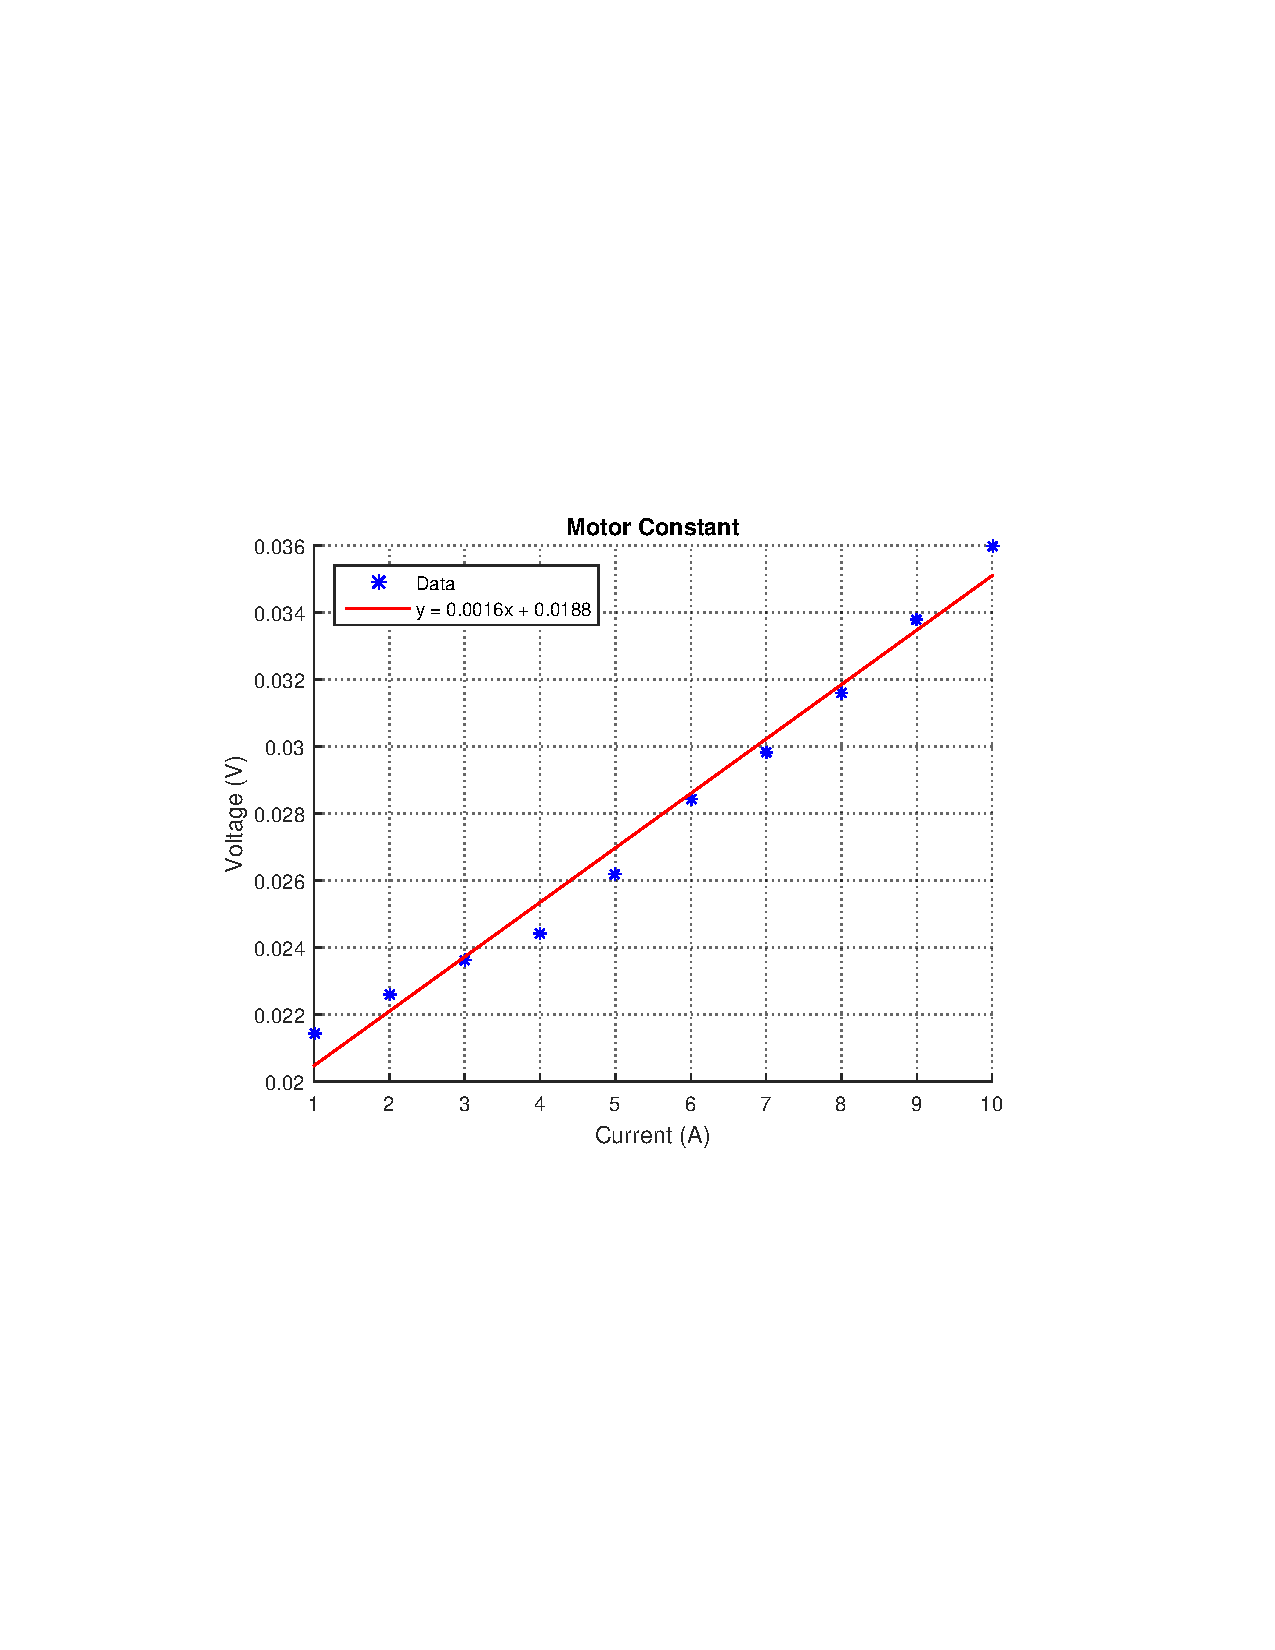
\includegraphics[width=\textwidth]{figures/motorConstant.pdf}
  }
	\caption{A plot of the torque at different currents, where the blue dots is the measurements and the red line is the least square line.}
	\label{motorConstant}
\end{figure}

The voltages measure are scaled by factor of 0,2 since the torque sensor outputs 5 V per \si{100N\cdot cm} giving a torque of 0,2 \si{N\cdot m/V} \cite{MWAW81P}.
After scaling the voltages to torques it is plotted and a lest square line is added as seen on \figref{motorConstant}. The relation between the current and torque is described as follows:

\begin{flalign}
  \eq{\tau}{K_t \cdot I_a}\unit{N\cdot m}\nonumber\\
  \eq{K_t} {\frac{\tau}{I_a}}\unit{N\cdot m \cdot A^{-1}}\nonumber
\end{flalign}
\hspace{6mm} Where:\\
\begin{tabular}{p{1cm}lll}
  & \si{\tau}   & is the torque                        &\unitWh{N\cdot m}\\
  & \si{I_a}    & is the current supplied to the motor &\unitWh{A}\\
  & \si{K_t}    & is the motor constant                &\unitWh{N\cdot m \cdot A^{-1}}
\end{tabular}

The value of \si{K_t} is then extracted directly as the slope of the least square regression:
\begin{flalign}
  \eq{K_t}{\num{0,0016}} \ \si{N\cdot m \cdot A^{-1}}&\nonumber
\end{flalign}
  \pagebreak
\subsubsection{Moment of Inertia} %\label{put a label here and uncomment}
\textbf{Name: Group 510}\\
\textbf{Date: 30/09 - 2015}

\subsubsection{Purpose}
The purpose of this test is to find the moment of inertia $I$, by measuring the motor velocity as a function of time.

\subsubsection{Setup}
Test setup

\subsubsection{List of Equipment}

\begin{table}[H]
\begin{tabular}{|l|l|p{4cm}|}
\hline%------------------------------------------------------------------------------------
  \textbf{Instrument}                        &  \textbf{AAU-no.}  &  \textbf{Type}       \\
\hline%------------------------------------------------------------------------------------
  Oscilloscope                               &  64672             &  Agilent DSO6034A    \\
\hline%------------------------------------------------------------------------------------
  Power Supply ($0 - 32$ V) ($0 - 10$ A)     &  77076             &  Ea - ps 7032 - 100  \\
\hline%------------------------------------------------------------------------------------
  Optical tachometer                         &  77087             &  Compact             \\
\hline%------------------------------------------------------------------------------------
\end{tabular}
\end{table}

\subsubsection{Procedure}

\begin{enumerate}
  \item Turn on the oscilloscope.
  \item On the oscilloscope press the "mode"-key choose the "normal"-option, set the trigger to "falling edge".
  \item To prevent false triggering on the oscilloscope set the trigger value to %\fxnote{input value from extracted data} mV with the turn-key.
  \item Turn on the power supply at 7 volt.
  \item Press "single"-key on oscilloscope and cut the power of the motor.
  \item Insert a USB-pin in the oscilloscope and press the save key to extract the data.
\end{enumerate}

\subsubsection{Results}

\begin{figure}[H]
	\centering
	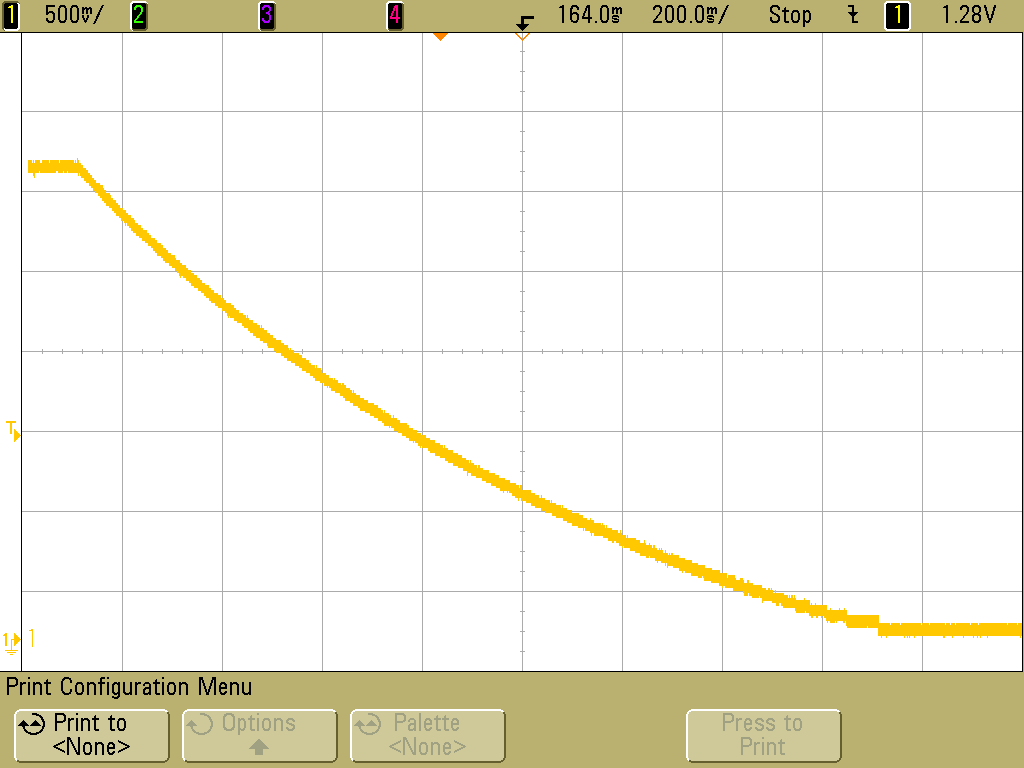
\includegraphics[scale=.4]{figures/Exercise7}
	\caption{Plot of test results}
\end{figure}
  \pagebreak
\subsection{Time Constant and Gain} %\label{put a label here and uncomment}
\textbf{Name: Group 510}\\
\textbf{Date: 30/09 - 2015}

\subsubsection{Purpose}
The purpose of this test is to find the motors time constant $\tau$ and gain. This is done by measuring the motors step response.

\subsubsection{Setup}
\begin{figure}[H]
  \centering
	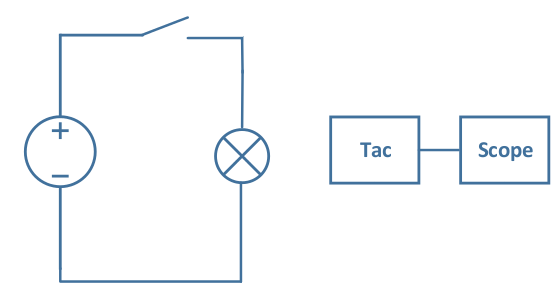
\includegraphics[scale=0.5]{figures/MotorTest8.png}
	\caption{Setup diagram}
\end{figure}

\subsubsection{List of Equipment}

\begin{table}[H]
\begin{tabular}{|l|l|p{4cm}|}
\hline%------------------------------------------------------------------------------------
  \textbf{Instrument}                        &  \textbf{AAU-no.}  &  \textbf{Type}       \\
\hline%------------------------------------------------------------------------------------
  Oscilloscope                               &  64672             &  Agilent DSO6034A    \\
\hline%------------------------------------------------------------------------------------
  Power Supply ($0 - 32$ V) ($0 - 10$ A)     &  77076             &  Ea - ps 7032 - 100  \\
\hline%------------------------------------------------------------------------------------
  Optical tachometer                         &  77087             &  Compact             \\
\hline%------------------------------------------------------------------------------------
\end{tabular}
\end{table}

\subsubsection{Procedure}

\begin{enumerate}
  \item Turn on the oscilloscope, and connect one channel to the power supply, and another to the tachometer.
  \item On the oscilloscope press the "trigger mode"-key choose the "normal"-option, set the trigger to "rising-edge", and the trigger source to the channel connected to the power supply.
  \item To prevent false triggering on the oscilloscope set the trigger value to \num{4,50}V with the turn-key.
  \item Press "single"-key on oscilloscope.
  \item Turn on the power supply at 5 volt.
  \item Insert a USB-flash drive in the oscilloscope and press the save key to extract the data.
\end{enumerate}

\subsubsection{Results}

\begin{figure}[H]
  \centering
  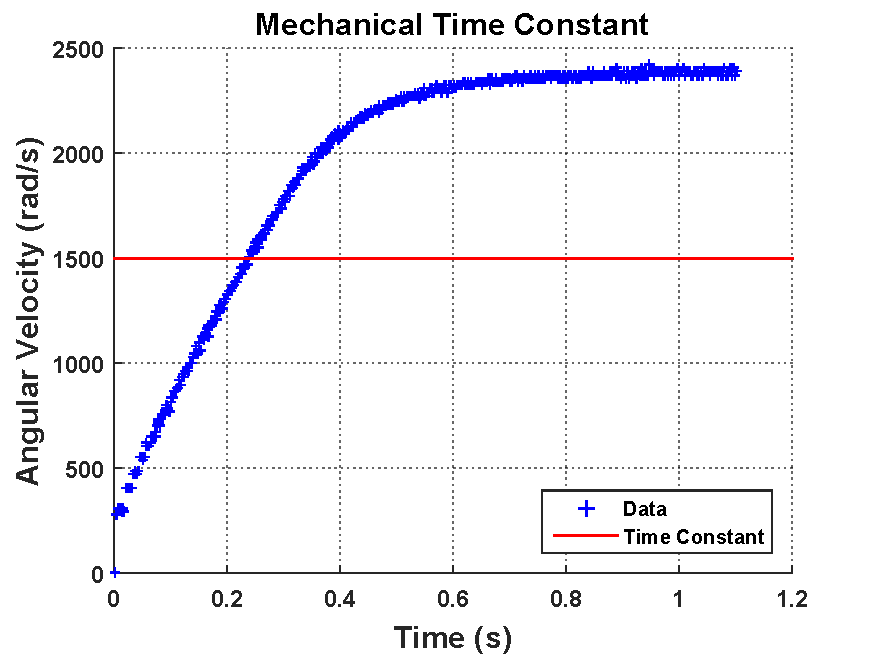
\includegraphics[width=.8\textwidth]{figures/mechanicalTimeConstant.pdf}
	\caption{A plot of the step response illustrating the angular velocity over time. The blue dots is the measurements and the red line indicates the mechanical time constant.}
	\label{mechanicalTimeConstant}
\end{figure}

The graph in \figref{mechanicalTimeConstant} shows the angular velocity of the motor over time. The read line shows the time constant at \si{\num{63.2} \%} of max angular velocity. In the data the mechanical time constant is found to be:
%
\begin{flalign}
  \eq{\tau_{mec}}{0,238} \tx{ s}&&\nonumber
\end{flalign}

\begin{figure}[H]
  \centering
 	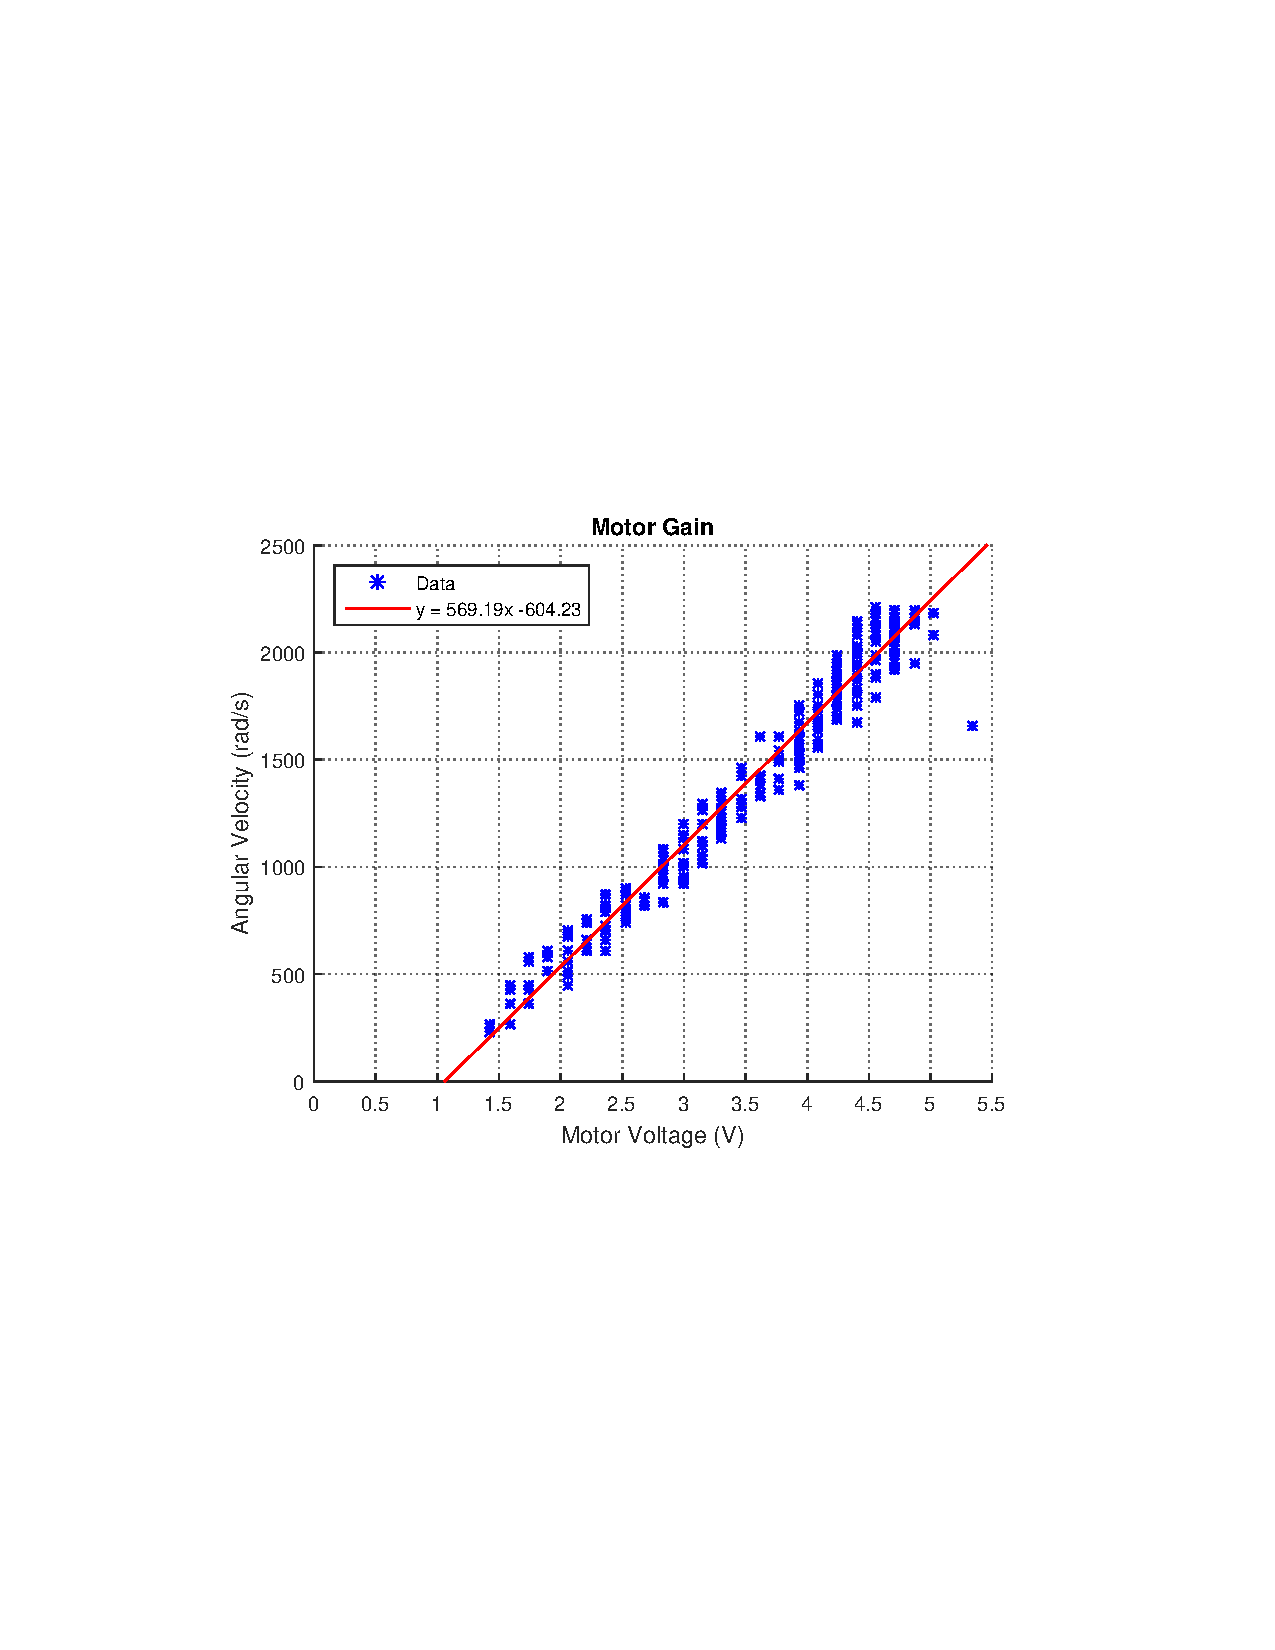
\includegraphics[width=.8\textwidth]{figures/motorGain.pdf}
  \caption{A plot of the motor's step response, where the input is motor voltage and the output is the angular velocity. The blue dots indicates the measurements and the red line is the tendency line.}
	\label{motorGain}
\end{figure}

The graph in \figref{motorGain} shows motor voltage in relation to the angular velocity, which reveals the gain, \si{K} of the system, as the slope of the least square regression line:
%
\begin{flalign}
  \eq{K}{\num{569.19}} \unit{\cdot}\nonumber
\end{flalign}


\printbibliography
\listoftodos

\end{document}